% IUT-Thesis v2.5

%CHANGE LOG IUT-Thesis v2.5
%---------------------------
%- Add some options to signature pages
%- Adaption to Texlive 2016, Xeperian 18.2 and Bidi 30.2
%- Fix some buges: paragraph footnote, reference style, and ...


% این قالب بر اساس فرمت پایان‌نامه‌ها و رساله‌های تحصیلات تکمیلی دانشگاه صنعتی اصفهان تهیه شده است. شما می‌توانید آخرین نسخه این قالب را از دریافت کنید.

% توصیه می‌شود که از توزیع تک‌لایو (TexLive) استفاده شود:
% http://tug.org/texlive/acquire-iso.html

% موفق باشید.
% محمد جان‌نثاری
% mohammad.jannesari@gmail.com
% امین فخاری
% a101.fakhari@gmail.com
% ‌فروردین 1396
% -----------------------------------------------------------------------------------

% نکات:

% برای دریافت نتیجه مطلوب از این قالب بایستی از آخرین نسخه تک‌لایو به همراه Xepersian نسخه 18.2 , Bidi نسخه 30.2 استفاده شود.

% برای آن‌که پردازش فایل و مشاهده خروجی در هنگام نوشتن پایان‌نامه آسان‌تر و سریع‌تر انجام شود، انجام موارد زیر توصیه می گردد:
% الف) فصل‌ها و بخش‌هایی که در حال نوشتن آن‌ها نیستید را غیر فعال کنید. به‌عنوان مثال، در این قالب، این دستورات را می‌توان در صورت عدم نیاز با اضافه کردن % به طور موقت غیرفعال کرد:
% \MakeTitlePage
% \MakeFarsiSignaturePage
% \clearpage
\thispagestyle{empty}
\newgeometry{left=3cm,right=4cm,top=7cm}

{\BZarScaleOne
{\fontsize{20pt}{0}\selectfont
\noindent
% عنوان تشکر و قدردانی---------------------------------------------------------
تشکر و قدردانی
% ؛---------------------------------------------------------
}}
\vspace{0.5cm}

{\BZarScaleOne
{\fontsize{12pt}{0.9cm}\selectfont % Zar 13
\noindent
% متن تشکر و قدردانی---------------------------------------------------------
سپاس خدای را که سخنوران، در ستودن او بمانند ...
% ؛---------------------------------------------------------
}}

\restoregeometry
% \MakeCopyRightPage
% \clearpage
\thispagestyle{empty}
\newgeometry{left=3cm,right=4cm,top=7cm}

{\BZarScaleOne
{\fontsize{28pt}{0}\selectfont
\noindent
% تقدیم اثر---------------------------------------------------------
{\normalsize تقدیم به}
\\[1cm]
\hspace*{1cm}
\centering{\textbf{\IrNasScaleOne\fontsize{54pt}{0}\selectfont ...}}
% ؛---------------------------------------------------------
}}
		
\restoregeometry
% \MakeTableOfContents
% \MakeListOfFigures
% \MakeListOfTables
% \MakeFarsiAbstract
% \input{Chapters/Chapter#}
% \MakeAppendices
% \section{مدیریت مراجع در لاتک}\label{App:RefMan}
در بخش \ref{Sec:Ref} اشاره شد که با دستور 
 \lr{\textbackslash bibitem}
  می‌توان یک مرجع را تعریف نمود و با فرمان
 \lr{\textbackslash cite}
  به آن ارجاع داد. این روش برای تعداد مراجع زیاد و تغییرات آنها مناسب نیست. در ادامه به صورت مختصر توضیحی در خصوص برنامه \lr{BibTeX} که همراه با توزیع‌های معروف تِک عرضه می‌شود و نحوه استفاده از آن در زی‌پرشین خواهیم داشت.

\subsection{ مدیریت مراجع با  \texorpdfstring{\lr{Bib\TeX}}{Bib\TeX} }
یکی از روش‌های قدرتمند و انعطاف‌پذیر برای نوشتن مراجع مقالات و مدیریت مراجع در لاتک، استفاده از  \lr{BibTeX} است.
 روش کار با  \lr{BibTeX} به این صورت است که مجموعه‌ی همه‌ی مراجعی را که در پروژه/پایان‌نامه/رساله استفاده کرده یا خواهیم کرد، 
در پرونده‌ی جداگانه‌ای نوشته و به آن فایل در سند خودمان به صورت مناسب لینک می‌دهیم.
 کنفرانس‌ها یا مجله‌های گوناگون برای نوشتن مراجع، قالب‌ها یا قراردادهای متفاوتی دارند که به آنها استیلهای مراجع گفته می‌شود.
 در این حالت به کمک ‌استیل‌های \lr{BibTeX} خواهید توانست تنها با تغییر یک پارامتر در پرونده‌ی ورودی خود، مراجع را مطابق قالب موردنظر تنظیم کنید. 
 بیشتر مجلات و کنفرانس‌های معتبر یک پرونده‌ی سبک (\lr{BibTeX Style}) با پسوند \lr{bst} در وب‌گاه خود می‌گذارند که برای همین منظور طراحی شده است.

به جز نوشتن مقالات این سبک‌ها کمک بسیار خوبی برای تهیه‌ی مستندات علمی همچون پایان‌نامه‌هاست که فرد می‌تواند هر قسمت از کارش را که نوشت مراجع مربوطه را به بانک مراجع خود اضافه نماید. با داشتن چنین بانکی از مراجع، وی خواهد توانست به راحتی یک یا چند ارجاع به مراجع و یا یک یا چند بخش را حذف یا اضافه ‌نماید؛ 
مراجع به صورت خودکار مرتب شده و فقط مراجع ارجاع داده شده در قسمت کتاب‌نامه خواهندآمد. قالب مراجع به صورت یکدست مطابق سبک داده شده بوده و نیازی نیست که کاربر درگیر قالب‌دهی به مراجع باشد. 
در این جا مجموعه‌ سبک‌های بسته \lr{Persian-bib} که برای  زی‌پرشین آماده شده‌اند به صورت مختصر معرفی شده و روش کار با آن‌ها گفته می‌شود. برای اطلاع بیشتر به راهنمای بسته‌ی \lr{Persian-bib} مراجعه فرمایید.
\subsection{سبک‌های فعلی قابل استفاده در زی‌پرشین}
در حال حاضر فایلهای سبک زیر برای استفاده در زی‌پرشین آماده شده‌اند:

\singlespacing
\begin{description}
\item [\lr{unsrt-fa.bst}] این سبک متناظر با \lr{unsrt.bst} می‌باشد. مراجع به ترتیب ارجاع در متن ظاهر می‌شوند.
\item [\lr{plain-fa.bst}] این سبک متناظر با \lr{plain.bst} می‌باشد. مراجع بر اساس نام‌خانوادگی نویسندگان، به ترتیب صعودی مرتب می‌شوند.
 همچنین ابتدا مراجع فارسی و سپس مراجع انگلیسی خواهند آمد.
\item [\lr{acm-fa.bst}] این سبک متناظر با \lr{acm.bst} می‌باشد. شبیه \lr{plain-fa.bst} است.  قالب مراجع کمی متفاوت است. اسامی نویسندگان انگلیسی با حروف بزرگ انگلیسی نمایش داده می‌شوند. (مراجع مرتب می‌شوند)
\item [\lr{ieeetr-fa.bst}] این سبک متناظر با \lr{ieeetr.bst} می‌باشد. (مراجع مرتب نمی‌شوند)
\item [\lr{plainnat-fa.bst}] این سبک متناظر با \lr{plainnat.bst} می‌باشد. نیاز به بسته \lr{natbib} دارد. (مراجع مرتب می‌شوند)
\item [\lr{chicago-fa.bst}] این سبک متناظر با \lr{chicago.bst} می‌باشد. نیاز به بسته \lr{natbib} دارد. (مراجع مرتب می‌شوند)
\item [\lr{asa-fa.bst}] این سبک متناظر با \lr{asa.bst} می‌باشد. نیاز به بسته \lr{natbib} دارد. (مراجع مرتب می‌شوند)
\item[\lr{ModifiedIEEEtranFa.bst}] این سبک متناظر با نحوه ارجاع در پایان‌نامه‌های دانشگاه صنعتی اصفهان می‌باشد.
\end{description}
\doublespacing

با استفاده از استیلهای فوق می‌توانید به انواع مختلفی از مراجع فارسی و لاتین ارجاع دهید. به عنوان نمونه مرجع 
\cite{Omidali82phdThesis}
 یک نمونه پروژه دکترا (به فارسی) و مرجع 
\cite{Vahedi87} یک نمونه مقاله مجله فارسی است.
مرجع 
\cite{Amintoosi87afzayesh}  یک نمونه  مقاله کنفرانس فارسی و
مرجع 
\cite{Pedram80osool} یک نمونه کتاب فارسی با ذکر مترجمان و ویراستاران فارسی است. مرجع 
\cite{Khalighi07MscThesis} یک نمونه پروژه کارشناسی ارشد انگلیسی و
\cite{Khalighi87xepersian} هم یک نمونه متفرقه  می‌باشند.
مراجع 
\cite{Gonzalez02book,Baker02limits} 
نمونه کتاب و مقاله انگلیسی هستند.

استیل مورد استفاده در این پروژه/پایان‌نامه/رساله 
\lr{ModifiedIEEEtranFa}
است که خروجی آنرا در بخش مراجع می‌توانید مشاهده کنید.
نمونه  خروجی سبک \lr{asa-fa} در شکل \ref{fig:asafa} آمده است.

\begin{figure}[t]
\centering
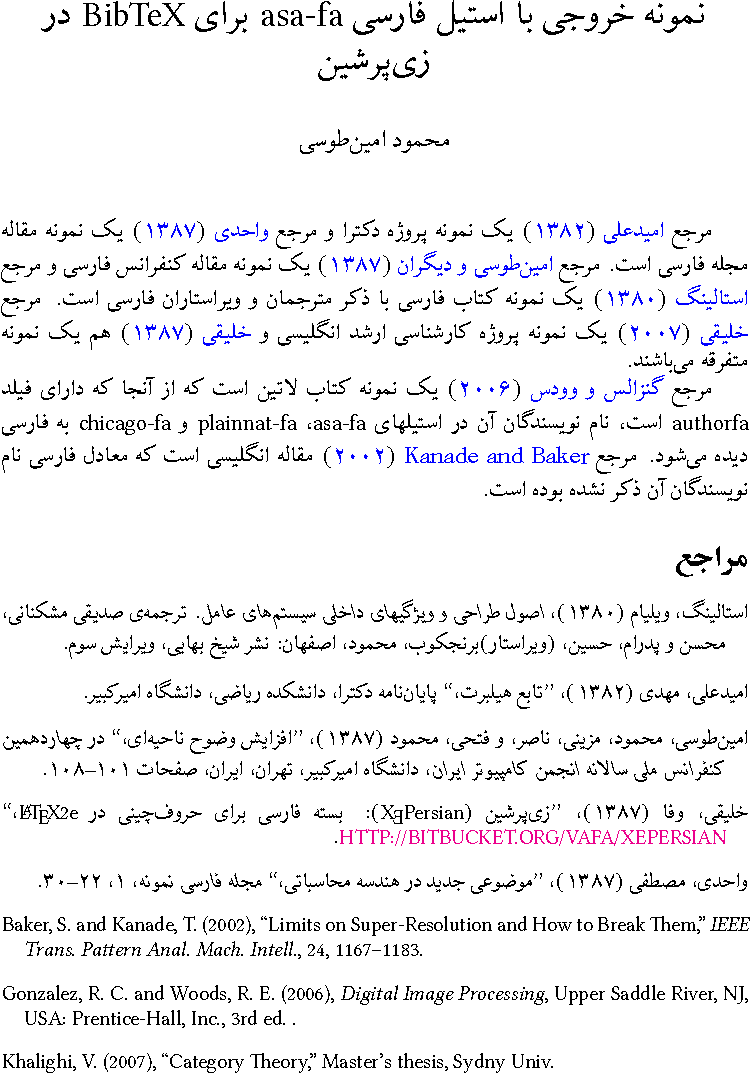
\includegraphics[width=.8\textwidth]{Figures/App1/asa-fa-crop.pdf}
\caption{نمونه خروجی با سبک \lr{asa-fa}}
\label{fig:asafa}
\end{figure} 
\subsection{ نحوه استفاده از سبک‌های فارسی}
برای استفاده از بیب‌تک باید مراجع خود را در یک فایل با پسوند \lr{bib} ذخیره نمایید. یک فایل \lr{bib} در واقع یک پایگاه داده از مراجع\LTRfootnote{Bibliography Database}  شماست که هر مرجع در آن به عنوان یک رکورد از این پایگاه داده
با قالبی خاص ذخیره می‌شود. به هر رکورد یک مدخل\LTRfootnote{Entry} گفته می‌شود. یک نمونه مدخل برای معرفی کتاب \lr{Digital Image Processing} در ادامه آمده است:

\singlespacing
\begin{LTR}
\begin{verbatim}
@BOOK{Gonzalez02image,
  AUTHOR =      {Rafael Gonzalez and Richard Woods},
  TITLE =       {Digital Image Processing},
  PUBLISHER =   {Prentice-Hall, Inc.},
  YEAR =        {2006},
  EDITION =     {3rd},
  ADDRESS =     {Upper Saddle River, NJ, USA}
}
\end{verbatim}
\end{LTR}
\doublespacing

در مثال فوق، \lr{@BOOK} مشخصه‌ی شروع یک مدخل مربوط به یک کتاب و \lr{Gonzalez02book} برچسبی است که به این مرجع منتسب شده است.
 این برچسب بایستی یکتا باشد. برای آنکه فرد به راحتی بتواند برچسب مراجع خود را به خاطر بسپارد و حتی‌الامکان برچسب‌ها متفاوت با هم باشند معمولاً از قوانین خاصی به این منظور استفاده می‌شود. یک قانون می‌تواند فامیل نویسنده‌ی اول+دورقم سال نشر+اولین کلمه‌ی عنوان اثر باشد. به \lr{AUTHOR} و $\dots$ و \lr{ADDRESS} فیلدهای این مدخل گفته می‌شود؛ که هر یک با مقادیر مربوط به مرجع مقدار گرفته‌اند. ترتیب فیلدها مهم نیست. 

انواع متنوعی از مدخل‌ها برای اقسام مختلف مراجع همچون کتاب، مقاله‌ی کنفرانس و مقاله‌ی ژورنال وجود دارد که برخی فیلدهای آنها با هم متفاوت است. 
نام فیلدها بیانگر نوع اطلاعات آن می‌باشد. مثالهای ذکر شده در فایل \lr{References.bib} کمک خوبی به شما خواهد بود. 
%این فایل یک فایل متنی بوده و با ویرایشگرهای معمول همچون \lr{Notepad++} قابل ویرایش می‌باشد. برنامه‌هایی همچون 
%\lr{TeXMaker}
% امکاناتی برای نوشتن این مدخل‌ها دارند و به صورت خودکار فیلدهای مربوطه را در فایل \lr{bib}  شما قرار می‌دهند.  
با استفاده از سبک‌های فارسی آماده شده، محتویات هر فیلد می‌تواند به فارسی نوشته شود، ترتیب مراجع و نحوه‌ی چینش فیلدهای هر مرجع را سبک مورد استفاده  مشخص خواهد کرد.

نکته: بدون اعمال تنظیمات موردنیاز \lr{Bib\TeX} در \lr{TeXWorks}، مراجع فارسی در استیل‌هایی که مراجع را به صورت مرتب شده چاپ می‌کنند، ترتیب کاملاً درستی نخواهند داشت. برای توضیحات بیشتر \cite{persianbib87userguide} را ببینید یا به سایت پارسی‌لاتک مراجعه فرمایید.

\textbf{برای درج مراجع خود لازم نیست نگران موارد فوق باشید. در فایل 
\lr{References.bib}
 که همراه با این پروژه/پایان‌نامه/رساله هست، موارد مختلفی درج شده است و کافیست مراجع خود را جایگزین موارد مندرج در آن نمایید.
}

پس از قرار دادن مراجع خود، یک بار \lr{XeLaTeX} را روی سند خود اجرا نمایید، سپس \lr{bibtex} و پس از آن دوبار \lr{XeLaTeX} را. در \lr{TeXstudio} کلید \lr{F8} و در \lr{TeXWorks} هم گزینه‌ی \lr{BibTeX} از منوی \lr{Typeset}، \lr{BibTeX} را روی سند شما اجرا می‌کنند.

برای بسیاری از مقالات لاتین حتی لازم نیست که مدخل مربوط به آنرا خودتان بنویسید. با جستجوی نام مقاله + کلمه \lr{bibtex}  در اینترنت سایتهای بسیاری همچون \lr{ACM} و \lr{ScienceDirect} را خواهید یافت که مدخل \lr{bibtex} مربوط به مقاله شما را دارند و کافیست آنرا به انتهای فایل \lr{References} اضافه کنید.

از هر یک از سبکهای \lr{Persian-bib} می‌توانید استفاده کنید، البته اگر از سه استیل آخر استفاده می‌کنید و مایلید که مراجع شما شماره بخورند باید بسته \lr{natbib} را با گزینه \lr{numbers} فراخوانی نمایید.
\newpage
\section{‌جدول، نمودار و الگوریتم در لاتک}\label{App:Latex:More}
در این بخش نمونه مثالهایی از جدول، نمودار و الگوریتم در لاتک را خواهیم دید.
\subsection{مدلهای حرکت دوبعدی}
بسیاری از اوقات حرکت بین دو تصویر از یک صحنه با یکی از مدلهای پارامتری ذکر شده در جدول \eqref{tab:MotionModels} قابل مدل نمودن می‌باشد.  
\begin{table}[ht]
	\caption{مدلهای تبدیل.}
	\label{tab:MotionModels}
	\centering
	\onehalfspacing
	\begin{tabular}{|r|c|l|r|}
		\hline نام مدل & درجه آزادی & تبدیل مختصات & توضیح \\ 
		\hline انتقالی & ۲ & $\begin{aligned} x'=x+t_x \\ y'=y+t_y \end{aligned}$  &  انتقال دوبعدی\\ 
		\hline اقلیدسی & ۳ & $\begin{aligned} x'=xcos\theta - ysin\theta+t_x \\ y'=xsin\theta+ycos\theta+t_y \end{aligned}$  &  انتقالی+دوران \\ 
		\hline مشابهت & ۴ & $\begin{aligned} x'=sxcos\theta - sysin\theta+t_x \\ y'=sxsin\theta+sycos\theta+t_y  \end{aligned}$  & اقلیدسی+تغییرمقیاس \\ 
		\hline آفین & ۶ & $\begin{aligned} x'=a_{11}x+a_{12}y+t_x \\ y'=a_{21}x+a_{22}y+t_y \end{aligned}$  & مشابهت+اریب‌شدگی \\ 
		\hline  پروجکتیو & ۸ & $\begin{aligned} x'&=(m_1x+m_2y+m_3)/D \\ y'&=(m_4x+m_5y+m_6)/D \\ D&=m_7x+m_8y+1 \end{aligned}$  & آفین+\lr{keystone+chirping} \\ 
		\hline  شارنوری & $\infty $ & $\begin{aligned} x'=x+v_x(x,y) \\ y'=y+v_y(x,y) \end{aligned}$  &  حرکت آزاد\\ 
		\hline 
	\end{tabular} 
\end{table}

\subsection{ماتریس}

شناخته‌شده‌ترین روش تخمین ماتریس هوموگرافی الگوریتم تبدیل خطی مستقیم (\lr{DLT\LTRfootnote{Direct Linear Transform}}) است.  فرض کنید چهار زوج نقطهٔ متناظر در دو تصویر در دست هستند،  $\mathbf{x}_i\leftrightarrow\mathbf{x}'_i$   و تبدیل با رابطهٔ
$\mathbf{x}'_i = H\mathbf{x}_i$
نشان داده می‌شود که در آن:
\[\mathbf{x}'_i=(x'_i,y'_i,w'_i)^\top  \]
و
\[ H=\left[
\begin{array}{ccc}
h_1 & h_2 & h_3 \\ 
h_4 & h_5 & h_6 \\ 
h_7 & h_8 & h_9
\end{array} 
\right]\]
رابطه زیر را برای الگوریتم  \eqref{alg:DLT} لازم دارم.
\begin{equation}\label{eq:DLT_Ah}
\left[
\begin{array}{ccc}
0^\top & -w'_i\mathbf{x}_i^\top & y'_i\mathbf{x}_i^\top \\ 
w'_i\mathbf{x}_i & 0^\top & -x'_i\mathbf{x}_i^\top \\ 
- y'_i\mathbf{x}_i^\top & x'_i\mathbf{x}_i^\top & 0^\top
\end{array} 
\right]
\left(
\begin{array}{c}
\mathbf{h}^1 \\ 
\mathbf{h}^2 \\ 
\mathbf{h}^3
\end{array} 
\right)=0
\end{equation}

\subsection{الگوریتم با دستورات فارسی}
با مفروضات فوق، الگوریتم \lr{DLT} به صورت نشان داده شده در الگوریتم \eqref{alg:DLT}  خواهد بود.
\begin{algorithm}[t]
	\onehalfspacing
	\caption{الگوریتم \lr{DLT} برای تخمین ماتریس هوموگرافی.} \label{alg:DLT}
	\begin{algorithmic}[1]
		\REQUIRE $n\geq4$ زوج نقطهٔ متناظر در دو تصویر 
		${\mathbf{x}_i\leftrightarrow\mathbf{x}'_i}$،\\
		\ENSURE ماتریس هوموگرافی $H$ به نحوی‌که: 
		$\mathbf{x}'_i = H \mathbf{x}_i$.
		\STATE برای هر زوج نقطهٔ متناظر
		$\mathbf{x}_i\leftrightarrow\mathbf{x}'_i$ 
		ماتریس $\mathbf{A}_i$ را با استفاده از رابطهٔ \ref{eq:DLT_Ah} محاسبه کنید.
		\STATE ماتریس‌های ۹ ستونی  $\mathbf{A}_i$ را در قالب یک ماتریس $\mathbf{A}$ ۹ ستونی ترکیب کنید. 
		\STATE تجزیهٔ مقادیر منفرد \lr{(SVD)}  ماتریس $\mathbf{A}$ را بدست آورید. بردار واحد متناظر با کمترین مقدار منفرد جواب $\mathbf{h}$ خواهد بود.
		\STATE  ماتریس هوموگرافی $H$ با تغییر شکل $\mathbf{h}$ حاصل خواهد شد.
	\end{algorithmic}
\end{algorithm}

\subsection{الگوریتم با دستورات لاتین}
الگوریتم \ref{alg:RANSAC} یک الگوریتم با دستورات لاتین است.

\begin{algorithm}[t]
	\onehalfspacing
	\caption{الگوریتم \lr{RANSAC} برای تخمین ماتریس هوموگرافی.} \label{alg:RANSAC}
	\begin{latin}
		\begin{algorithmic}[1]
			\REQUIRE $n\geq4$ putative correspondences, number of estimations, $N$, distance threshold $T_{dist}$.\\
			\ENSURE Set of inliers and Homography matrix $H$.
			\FOR{$k = 1$ to $N$}
			\STATE Randomly choose 4 correspondence,
			\STATE Check whether these points are colinear, if so, redo the above step
			\STATE Compute the homography $H_{curr}$ by DLT algorithm from the 4 points pairs,
			\STATE $\ldots$ % الگوریتم کامل نیست
			\ENDFOR
			\STATE Refinement: re-estimate H from all the inliers using the DLT algorithm.
		\end{algorithmic}
	\end{latin}
\end{algorithm}

\subsection{نمودار}
لاتک بسته‌هایی با قابلیت‌های زیاد برای رسم انواع مختلف نمودارها دارد. مانند بسته‌های \lr{Tikz} و  \lr{PSTricks}. توضیح اینها فراتر از این پیوست کوچک است. مثالهایی از رسم نمودار را در مجموعه پارسی‌لاتک خواهید یافت. توصیه می‌کنم که حتماً مثالهایی از برخی از آنها را ببینید. راهنمای همه آنها در تک‌لایو هست. نمونه مثالهایی از بسته \lr{Tikz} را می‌توانید در \url{http://www.texample.net/tikz/examples/} ببینید.

\subsection{تصویر}
نمونه تصاویری در بخش قبل دیدیم. دو تصویر شیر کنار هم را هم در شکل \ref{fig:twolion} مشاهده می‌کنید.
\begin{figure}[t]
	\centering 
	\subfloat[شیر ۱]{ \label{fig:twolion:one}
		
\includegraphics[width=.3\textwidth]{Figures/Ch2/lion.jpg}}
	%\hspace{2mm}
	\subfloat[شیر ۲]{ \label{fig:twolion:two}
		
\includegraphics[width=.3\textwidth]{Figures/Ch2/lion.jpg}}
	\caption{دو شیر}
	\label{fig:twolion} %% label for entire figure
\end{figure}
% \MakeEnglishAbstract
% \MakeEnglishSignaturePage
% ب) از گزینه draft برای فراخوانی کلاس استفاده کنید. یعنی
% \documentclass[a4paper,fleqn,10pt,oneside,draft]{book}
% این گزینه حالت چرکنویس را ایفا می‌کند و بر روی بسته‌های مختلف اثرهای متفاوتی دارد. به‌عنوان مثال: به جای شکل، تنها چهارچوب آن نمایش داده شود، لینک‌های hyperref غیر فعال گردد، فایل‌های خارجی را در بسته listings اضافه نمی‌کند و ... و همه این موارد سبب کاهش زمان اجرا و حجم فایل می‌شود.

% در صورتی که میخواهید به سطر بعد بروید اما نمیخواهید بین دو کلمه‌ای که نوشتید فاصله بیفتد کافی است در انتهای خط اول  (بدون فاصله) کاراکتر % را اضافه کنید. با این عمل، لاتک خط فاصله ایجاد شده در اثر تغییر سطر را به عنوان توضیح اضافه یا کامنت در نظر میگیرد و در خروجی اعمال نمی‌کند.

% توصیه می‌شود از شکل‌های برداری با فرمت PDF استفاده شود. این کار علاوه بر افزایش کیفیت رسال/پایان‌نامه/گزارش، باعث کاهش حجم شکل‌ها (و در نتیجه  کاهش حجم فایل نهایی) و همچنین کاهش زمان پردازش می‌شود.

% در این قالب سعی شده است که از تمامی بخش‌های موجود در پایان‌نامه‌ها نمونه‌ای آورده شود.

% لطفا هرگونه عدم تطابق این قالب با فرمت دانشگاه صنعتی اصفهان را به ایمیل (mohammad.jannesari@gmail.com) اطلاع دهید.

\documentclass[a4paper,fleqn,10pt,oneside]{book}
\usepackage{Settings/IUT-Thesis}
%-----------------------------
% دستورهای مورد نیاز را در این قسمت اضافه نمایید:
\allowdisplaybreaks
%-----------------------------

\begin{document}

\pagestyle{plain}
\pagenumbering{adadi}
\setcounter{page}{2}

% ░░░░░░░▒▒▒▒▒▒▓▓▓▓ In the Name of Allah ▓▓▓▓▒▒▒▒▒▒░░░░░░░
\clearpage
\thispagestyle{empty}
\begin{figure}[t]
\centering

\includegraphics[scale=1.3]{Settings/Allah.pdf}
\end{figure}

% ░░░░░░░▒▒▒▒▒▒▓▓▓▓ Title Page ▓▓▓▓▒▒▒▒▒▒░░░░░░░
\DepartmentFa{دانشکده مهندسی مکانیک}
\ThesisTypeFa{پایان‌نامه} % Or \ThesisTypeFa{رساله} Or \ThesisTypeFa{پیشنهادیه پایان‌نامه}
\DegreeFa{کارشناسی ارشد} % Or \DegreeFa{دکتری} 
\FieldFa{مهندسی مکانیک}
\YourFullnameFa{محمد جان‌نثاری}
\FirstSupervisorFa{دکتر محمود کدخدایی}
\SecondSupervisorFa{دکتر پیمان مصدق} % Optional (Remove It If You Don't Have)
\YearFa{1395}
\TitleFa{
مدل‌سازی اجزای محدود رفتار بیومکانیکی بافت کره چشم  
\\[0.4cm]
با استفاده از فشار داخلی چشم
}
% اگر عنوان رساله طولانی بود، در دو خط به صورت نشان داده شده تقسیم شود.

\MakeTitlePage%

% ░░░░░░░▒▒▒▒▒▒▓▓▓▓ Signature - Farsi ▓▓▓▓▒▒▒▒▒▒░░░░░░░
\Prefix{آقای} %\Prefix{خانم}
\DateFa{1395/10/20}
%\FirstAdvisorFa{دکتر مشاور اول} % Optional (Remove It If You Don't Have)
%\SecondAdvisorFa{دکتر مشاور دوم} % Optional (Remove It If You Don't Have)
\FirstExaminerFa{دکتر داور اول} % Optional (Remove It If You Don't Have)
\SecondExaminerFa{دکتر داور دوم} % Optional (Remove It If You Don't Have)
%\ThirdExaminerFa{دکتر داور سوم} % Optional (Remove It If You Don't Have)
%\FourthExaminerFa{دکتر داور چهارم} % Optional (Remove It If You Don't Have)
%\FifthExaminerFa{دکتر داور پنجم} % Optional (Remove It If You Don't Have)
\DeanOfDepartmentFa{دکتر تحصیلات تکمیلی دانشکده}

\MakeFarsiSignaturePage%

% ░░░░░░░▒▒▒▒▒▒▓▓▓▓ Acknowledgments ▓▓▓▓▒▒▒▒▒▒░░░░░░░
\clearpage
\thispagestyle{empty}
\newgeometry{left=3cm,right=4cm,top=7cm}

{\BZarScaleOne
{\fontsize{20pt}{0}\selectfont
\noindent
% عنوان تشکر و قدردانی---------------------------------------------------------
تشکر و قدردانی
% ؛---------------------------------------------------------
}}
\vspace{0.5cm}

{\BZarScaleOne
{\fontsize{12pt}{0.9cm}\selectfont % Zar 13
\noindent
% متن تشکر و قدردانی---------------------------------------------------------
سپاس خدای را که سخنوران، در ستودن او بمانند ...
% ؛---------------------------------------------------------
}}

\restoregeometry%

% ░░░░░░░▒▒▒▒▒▒▓▓▓▓ CopyRight ▓▓▓▓▒▒▒▒▒▒░░░░░░░
\MakeCopyRightPage%

% ░░░░░░░▒▒▒▒▒▒▓▓▓▓ Dedication ▓▓▓▓▒▒▒▒▒▒░░░░░░░
\clearpage
\thispagestyle{empty}
\newgeometry{left=3cm,right=4cm,top=7cm}

{\BZarScaleOne
{\fontsize{28pt}{0}\selectfont
\noindent
% تقدیم اثر---------------------------------------------------------
{\normalsize تقدیم به}
\\[1cm]
\hspace*{1cm}
\centering{\textbf{\IrNasScaleOne\fontsize{54pt}{0}\selectfont ...}}
% ؛---------------------------------------------------------
}}
		
\restoregeometry%

% ░░░░░░░▒▒▒▒▒▒▓▓▓▓ Table of Contents/Figures/Tables ▓▓▓▓▒▒▒▒▒▒░░░░░░░
\MakeTableOfContents%
\MakeListOfFigures%
\MakeListOfTables%
\MakeListOfAlgorithms% for test

% ----------------------------------------------------------------------------
\clearpage
\pagestyle{myheadings}
\pagenumbering{arabic}
\setcounter{page}{1}

% ░░░░░░░▒▒▒▒▒▒▓▓▓▓ Abstract - Farsi ▓▓▓▓▒▒▒▒▒▒░░░░░░░
\AbstractFa{
در این قسمت چکیده‌ی فارسی پایان‌نامه نوشته می‌شود. در این قسمت چکیده‌ی فارسی پایان‌نامه نوشته می‌شود. در این قسمت چکیده‌ی فارسی پایان‌نامه نوشته می‌شود. در این قسمت چکیده‌ی فارسی پایان‌نامه نوشته می‌شود. در این قسمت چکیده‌ی فارسی پایان‌نامه نوشته می‌شود. در این قسمت چکیده‌ی فارسی پایان‌نامه نوشته می‌شود. در این قسمت چکیده‌ی فارسی پایان‌نامه نوشته می‌شود. در این قسمت چکیده‌ی فارسی پایان‌نامه نوشته می‌شود. در این قسمت چکیده‌ی فارسی پایان‌نامه نوشته می‌شود. در این قسمت چکیده‌ی فارسی پایان‌نامه نوشته می‌شود. در این قسمت چکیده‌ی فارسی پایان‌نامه نوشته می‌شود. در این قسمت چکیده‌ی فارسی پایان‌نامه نوشته می‌شود. در این قسمت چکیده‌ی فارسی پایان‌نامه نوشته می‌شود. در این قسمت چکیده‌ی فارسی پایان‌نامه نوشته می‌شود. در این قسمت چکیده‌ی فارسی پایان‌نامه نوشته می‌شود. در این قسمت چکیده‌ی فارسی پایان‌نامه نوشته می‌شود. در این قسمت چکیده‌ی فارسی پایان‌نامه نوشته می‌شود. در این قسمت چکیده‌ی فارسی پایان‌نامه نوشته می‌شود. در این قسمت چکیده‌ی فارسی پایان‌نامه نوشته می‌شود. در این قسمت چکیده‌ی فارسی پایان‌نامه نوشته می‌شود. در این قسمت چکیده‌ی فارسی پایان‌نامه نوشته می‌شود. در این قسمت چکیده‌ی فارسی پایان‌نامه نوشته می‌شود. در این قسمت چکیده‌ی فارسی پایان‌نامه نوشته می‌شود. در این قسمت چکیده‌ی فارسی پایان‌نامه نوشته می‌شود. در این قسمت چکیده‌ی فارسی پایان‌نامه نوشته می‌شود. در این قسمت چکیده‌ی فارسی پایان‌نامه نوشته می‌شود. در این قسمت چکیده‌ی فارسی پایان‌نامه نوشته می‌شود. در این قسمت چکیده‌ی فارسی پایان‌نامه نوشته می‌شود. در این قسمت چکیده‌ی فارسی پایان‌نامه نوشته می‌شود. در این قسمت چکیده‌ی فارسی پایان‌نامه نوشته می‌شود.‎‎
}

\KeywordsFa{
کلمه‌ی کليدی اوّل،  کلمه‌ی کليدی دوم ، کلمه‌ی کليدی سوم،  کلمه‌ی کليدی چهارم، کلمه‌ی کليدی پنجم
}%
\MakeFarsiAbstract%

% ░░░░░░░▒▒▒▒▒▒▓▓▓▓ Chapters ▓▓▓▓▒▒▒▒▒▒░░░░░░░
\clearpage
\baselineskip=0.9cm

\chapter{راهنمای استفاده از کلاس}
\section{مقدمه}
حروف‌چینی پروژه کارشناسی، پایان‌نامه یا رساله یکی از موارد پرکاربرد استفاده از زی‌پرشین\cite{Khalighi87xepersian} است.  یک پروژه، پایان‌نامه یا رساله،  احتیاج به تنظیمات زیادی از نظر صفحه‌آرایی  دارد که وقت زیادی از دانشجو می‌گیرد.به دلیل قابلیت‌های بسیار لاتک در حروف‌چینی، یک کلاس با نام 
\lr{IUT-Thesis}
برای حروف‌چینی پروژه‌ها، پایان‌نامه‌ها و رساله‌های دانشگاه صنعتی اصفهان با استفاده از نرم‌افزار زی‌پرشین،  آماده شده است. این فایل به 
گونه‌ای طراحی شده است که کلیات خواسته‌های مورد نیاز  مدیریت تحصیلات تکمیلی دانشگاه صنعتی اصفهان \cite{IUTThesisGuide} را برآورده می‌کند.% و نیز، حروف‌چینی بسیاری از قسمت‌های آن، به طور خودکار انجام می‌شود.

راهنمای نگارش پایان‌نامه دانشگاه صنعتی اصفهان به دو مقوله می‌پردازد، اول قالب و چگونگی صفحه‌آرایی پایان‌نامه، مانند اندازه و نوع قلم بخشهای مختلف، چینش فصلها، قالب مراجع و مواردی از این قبیل و دوم محتوای هر فصل پایان‌نامه. 
درصورت استفاده از این کلاس، دانشجو  نیازی نیست که نگران مقوله اول باشد. لاتک همه کارها را برای وی انجام می‌دهد. فقط کافیست مطالب خود را تایپ و سند خود را با لاتک و ابزار آن اجرا کند تا پایان‌نامه خود را با قالب دانشگاه داشته باشد.
کلیه فایل‌های لازم برای حروف‌چینی با کلاس گفته شده، داخل پوشه‌ای به نام
\lr{IUT-Thesis}
قرار داده شده است. توجه داشته باشید که برای استفاده از این کلاس باید فونت‌های
\lr{Times New Roman}،
\lr{B Zar}
و
\lr{IranNastaliq}
روی سیستم شما نصب شده باشد.
\section{این همه فایل؟!}\label{sec2}
از آنجایی که یک پایان‌نامه یا رساله، یک نوشته بلند محسوب می‌شود، لذا اگر همه تنظیمات و مطالب پایان‌نامه را داخل یک فایل قرار بدهیم، باعث شلوغی
و سردرگمی می‌شود. به همین خاطر، قسمت‌های مختلف پایان‌نامه یا رساله  داخل فایل‌های جداگانه قرار گرفته است. مثلاً تنظیمات پایه‌ای کلاس، داخل فایل
\lr{Settings\textbackslash IUT-Thesis.cls}، 
قسمت مشخصات فارسی پایان‌نامه، داخل 
\lr{IUT-Thesis.tex}،
مطالب فصل اول، داخل 
\lr{Chapters\textbackslash Chapter1.tex}
و ... قرار داده شده است. نکته مهمی که در اینجا وجود دارد این است که از بین این  فایل‌ها، فقط فایل 
\lr{IUT-Thesis.tex}
قابل اجرا است. یعنی بعد از تغییر فایل‌های دیگر، برای دیدن نتیجه تغییرات، باید این فایل را اجرا کرد. بقیه فایل‌ها به این فایل، کمک می‌کنند تا بتوانیم خروجی کار را ببینیم. اگر به فایل 
\lr{IUT-Thesis.tex}
دقت کنید، متوجه می‌شوید که قسمت‌های مختلف پایان‌نامه، توسط دستورهایی مانند 
\lr{input}
و
\lr{include}
به فایل اصلی، یعنی 
\lr{IUT-Thesis.tex}
معرفی شده‌اند. بنابراین، فایلی که همیشه با آن سروکار داریم، فایل 
\lr{IUT-Thesis.tex}
است.
در این فایل، فرض شده است که پایان‌نامه یا رساله شما، از دو فصل و دو پیوست، تشکیل شده است. با این حال، خودتان می‌توانید به راحتی فصل‌ها و پیوست‌های بیشتر را به این مجموعه، اضافه کنید. این کار، بسیار ساده است. فرض کنید بخواهید یک فصل دیگر هم به پایان‌نامه، اضافه کنید. برای این کار، کافی است یک فایل با نام دلخواه مثلاً 
\lr{Chapter3}
و با پسوند 
\lr{.tex}
بسازید و آن را داخل پوشه 
\lr{Chapters}
قرار دهید و سپس این فایل را با دستور 
\verb!\chapter{امتحانی}
\section{نمرات}
سلام سلام سلام%
\LTRfootnote{hello}
\LTRfootnote{hi}
\begin{itemize}
	\item یک
	\item دو
\end{itemize}

\%13 

\begin{equation}
\frac{1}{2}
\end{equation}

$2$

مرجع های 
\cite{Amintoosi09regional,Baker02limits}

!
داخل فایل
\lr{IUT-Thesis.tex}
قرار دهید.
\section{از کجا شروع کنم؟}
قبل از هر چیز، باید یک توزیع تِک مناسب مانند تک‌لایو
\lr{(TeXLive)}
را روی سیستم خود نصب کنید. تک‌لایو  را می‌توانید از 
\href{http://www.tug.org/texlive}{سایت رسمی آن}%
\LTRfootnote{http://www.tug.org/texlive}
دانلود کنید. 

برای تایپ و پردازش اسناد لاتک باید از یک ویرایشگر مناسب استفاده کنید. به همراه تک‌لایو ویرایشگر \lr{TeXstudio} هست که می‌توانید از آن برای پردازش اسناد خود استفاده کنید. 
ویرایش‌گر 
\lr{TeXstudio}
امکانات بیشتری دارد که آن را می‌توانید  از 
\href{http://http://www.texstudio.org}{سایت رسمی آن}
\LTRfootnote{http://http://www.texstudio.org}
دانلود کنید%
\footnote{توضیحات بیشتر درخصوص چگونگی اجرای اسناد زی‌پرشین را می‌توانید در فایل راهنمای زی‌پرشین ببینید.}.
در مرحله بعد، سعی کنید که  یک پشتیبان از پوشه 
\lr{IUT-Thesis}
بگیرید و آن را در یک جایی از هارددیسک سیستم خود ذخیره کنید تا در صورت خراب کردن فایل‌هایی که در حال حاضر، با آن‌ها کار می‌کنید، همه چیز را از 
دست ندهید.

حال اگر نوشتن پروژه/پایان‌نامه/رساله اولین تجربه شما از کار با لاتک است، توصیه می‌شود که یک‌بار به صورت اجمالی، کتاب «%
\href{http://www.tug.ctan.org/tex-archive/info/lshort/persian/lshort.pdf}{مقدمه‌ای نه چندان کوتاه بر
	\lr{\LaTeXe}}\footnote{اگر تک‌لایو کامل را داشته باشید، این کتاب را هم دارید. در هر صورت از آدرس زیر قابل دانلود است:\\
	\lr{\url{http://www.tug.ctan.org/tex-archive/info/lshort/persian/lshort.pdf}\hfill}}»
ترجمه دکتر مهدی امیدعلی را مطالعه کنید. این کتاب، کتاب بسیار کاملی است که خیلی از نیازهای شما در ارتباط با حروف‌چینی را برطرف می‌کند.
اگر عجله دارید، برخی دستورات پایه‌ای مورد نیاز در فصل \ref{Chap:latexIntro} بیان شده‌اند.


بعد از موارد گفته شده، فایل 
\lr{IUT-Thesis.tex}
را باز کنید و مشخصات فارسی و انگلیسی پایان‌نامه خود مثل نام، نام خانوادگی، عنوان پایان‌نامه، اسامی اساتید راهنما و مشاور، اسامی هیئت داوران و ... را جایگزین مشخصات موجود در فایل
\lr{IUT-Thesis.tex}
کنید. دقت داشته باشید که نیازی نیست 
نگران چینش این مشخصات در فایل پی‌دی‌اف خروجی باشید. فایل 
\lr{IUT-Thesis.cls}
همه این کارها را به طور خودکار برای شما انجام می‌دهد. در ضمن، موقع تغییر دادن دستورهای داخل فایل
\lr{IUT-Thesis.tex}
کاملاً دقت کنید. این دستورها، خیلی حساس هستند و ممکن است با یک تغییر کوچک، موقع اجرا، خطا بگیرید. برای دیدن خروجی کار، فایل 
\lr{IUT-Thesis.tex}
را 
\lr{Save}، 
(نه 
\lr{Save As})
کنید و بعد آن را اجرا کنید%
\footnote{فایلهای این مجموعه به گونه‌ای هستند که در \lr{TeXWorks}  بدون برگشتن به فایل اصلی، می‌توانید سند خود را اجرا کنید. }.

برای راحتی بیشتر، 
فایل 
\lr{IUT-Thesis.tex}
طوری طراحی شده است که کافی است فقط  یک‌بار مشخصات پروژه/پایان‌نامه/رساله  را وارد کنید. هر جای دیگر که لازم به درج این مشخصات باشد، این مشخصات به طور خودکار درج می‌شود. با این حال، اگر مایل بودید، می‌توانید تنظیمات موجود را تغییر دهید. توجه داشته باشید که اگر کاربر مبتدی هستید و یا با ساختار فایل‌های  
\lr{cls}
آشنایی ندارید، به هیچ وجه به فایل 
\lr{IUT-Thesis.cls}
دست نزنید.
\section[مطالب پروژه را چطور بنویسم؟]
{مطالب پروژه/پایان‌نامه/رساله را چطور بنویسم؟}
در این بخش در مورد نحوه نگارش مطالب صحبت می‌شود.
\subsection{نوشتن فصل‌ها}
همان‌طور که در بخش \ref{sec2} گفته شد، برای جلوگیری از شلوغی و سردرگمی کاربر در هنگام حروف‌چینی، قسمت‌های مختلف پروژه/پایان‌نامه/رساله از جمله فصل‌ها، در فایل‌های جداگانه‌ای قرار داده شده‌اند. 
بنابراین، اگر می‌خواهید مثلاً مطالب فصل ۱ را تایپ کنید، باید فایل‌های 
\lr{IUT-Thesis.tex}
و
\lr{Chapters\textbackslash Chapter1.tex}
را باز کنید و مطالب خود را جایگزین محتویات داخل فایل 
\lr{Chapters\textbackslash Chapter1.tex}
نمایید. 

نکته بسیار مهمی که در اینجا باید گفته شود این است که سیستم \lr{\TeX}، محتویات یک فایل تِک را به ترتیب پردازش می‌کند.  بنابراین، اگر مثلاً  دو فصل اول خود را نوشته و خروجی آنها را دیده‌اید و مشغول تایپ مطالب فصل ۳ هستید، بهتر است
که دو دستور 
\verb!\chapter{راهنمای استفاده از کلاس}
\section{مقدمه}
حروف‌چینی پروژه کارشناسی، پایان‌نامه یا رساله یکی از موارد پرکاربرد استفاده از زی‌پرشین\cite{Khalighi87xepersian} است.  یک پروژه، پایان‌نامه یا رساله،  احتیاج به تنظیمات زیادی از نظر صفحه‌آرایی  دارد که وقت زیادی از دانشجو می‌گیرد.به دلیل قابلیت‌های بسیار لاتک در حروف‌چینی، یک کلاس با نام 
\lr{IUT-Thesis}
برای حروف‌چینی پروژه‌ها، پایان‌نامه‌ها و رساله‌های دانشگاه صنعتی اصفهان با استفاده از نرم‌افزار زی‌پرشین،  آماده شده است. این فایل به 
گونه‌ای طراحی شده است که کلیات خواسته‌های مورد نیاز  مدیریت تحصیلات تکمیلی دانشگاه صنعتی اصفهان \cite{IUTThesisGuide} را برآورده می‌کند.% و نیز، حروف‌چینی بسیاری از قسمت‌های آن، به طور خودکار انجام می‌شود.

راهنمای نگارش پایان‌نامه دانشگاه صنعتی اصفهان به دو مقوله می‌پردازد، اول قالب و چگونگی صفحه‌آرایی پایان‌نامه، مانند اندازه و نوع قلم بخشهای مختلف، چینش فصلها، قالب مراجع و مواردی از این قبیل و دوم محتوای هر فصل پایان‌نامه. 
درصورت استفاده از این کلاس، دانشجو  نیازی نیست که نگران مقوله اول باشد. لاتک همه کارها را برای وی انجام می‌دهد. فقط کافیست مطالب خود را تایپ و سند خود را با لاتک و ابزار آن اجرا کند تا پایان‌نامه خود را با قالب دانشگاه داشته باشد.
کلیه فایل‌های لازم برای حروف‌چینی با کلاس گفته شده، داخل پوشه‌ای به نام
\lr{IUT-Thesis}
قرار داده شده است. توجه داشته باشید که برای استفاده از این کلاس باید فونت‌های
\lr{Times New Roman}،
\lr{B Zar}
و
\lr{IranNastaliq}
روی سیستم شما نصب شده باشد.
\section{این همه فایل؟!}\label{sec2}
از آنجایی که یک پایان‌نامه یا رساله، یک نوشته بلند محسوب می‌شود، لذا اگر همه تنظیمات و مطالب پایان‌نامه را داخل یک فایل قرار بدهیم، باعث شلوغی
و سردرگمی می‌شود. به همین خاطر، قسمت‌های مختلف پایان‌نامه یا رساله  داخل فایل‌های جداگانه قرار گرفته است. مثلاً تنظیمات پایه‌ای کلاس، داخل فایل
\lr{Settings\textbackslash IUT-Thesis.cls}، 
قسمت مشخصات فارسی پایان‌نامه، داخل 
\lr{IUT-Thesis.tex}،
مطالب فصل اول، داخل 
\lr{Chapters\textbackslash Chapter1.tex}
و ... قرار داده شده است. نکته مهمی که در اینجا وجود دارد این است که از بین این  فایل‌ها، فقط فایل 
\lr{IUT-Thesis.tex}
قابل اجرا است. یعنی بعد از تغییر فایل‌های دیگر، برای دیدن نتیجه تغییرات، باید این فایل را اجرا کرد. بقیه فایل‌ها به این فایل، کمک می‌کنند تا بتوانیم خروجی کار را ببینیم. اگر به فایل 
\lr{IUT-Thesis.tex}
دقت کنید، متوجه می‌شوید که قسمت‌های مختلف پایان‌نامه، توسط دستورهایی مانند 
\lr{input}
و
\lr{include}
به فایل اصلی، یعنی 
\lr{IUT-Thesis.tex}
معرفی شده‌اند. بنابراین، فایلی که همیشه با آن سروکار داریم، فایل 
\lr{IUT-Thesis.tex}
است.
در این فایل، فرض شده است که پایان‌نامه یا رساله شما، از دو فصل و دو پیوست، تشکیل شده است. با این حال، خودتان می‌توانید به راحتی فصل‌ها و پیوست‌های بیشتر را به این مجموعه، اضافه کنید. این کار، بسیار ساده است. فرض کنید بخواهید یک فصل دیگر هم به پایان‌نامه، اضافه کنید. برای این کار، کافی است یک فایل با نام دلخواه مثلاً 
\lr{Chapter3}
و با پسوند 
\lr{.tex}
بسازید و آن را داخل پوشه 
\lr{Chapters}
قرار دهید و سپس این فایل را با دستور 
\verb!\chapter{امتحانی}
\section{نمرات}
سلام سلام سلام%
\LTRfootnote{hello}
\LTRfootnote{hi}
\begin{itemize}
	\item یک
	\item دو
\end{itemize}

\%13 

\begin{equation}
\frac{1}{2}
\end{equation}

$2$

مرجع های 
\cite{Amintoosi09regional,Baker02limits}

!
داخل فایل
\lr{IUT-Thesis.tex}
قرار دهید.
\section{از کجا شروع کنم؟}
قبل از هر چیز، باید یک توزیع تِک مناسب مانند تک‌لایو
\lr{(TeXLive)}
را روی سیستم خود نصب کنید. تک‌لایو  را می‌توانید از 
\href{http://www.tug.org/texlive}{سایت رسمی آن}%
\LTRfootnote{http://www.tug.org/texlive}
دانلود کنید. 

برای تایپ و پردازش اسناد لاتک باید از یک ویرایشگر مناسب استفاده کنید. به همراه تک‌لایو ویرایشگر \lr{TeXstudio} هست که می‌توانید از آن برای پردازش اسناد خود استفاده کنید. 
ویرایش‌گر 
\lr{TeXstudio}
امکانات بیشتری دارد که آن را می‌توانید  از 
\href{http://http://www.texstudio.org}{سایت رسمی آن}
\LTRfootnote{http://http://www.texstudio.org}
دانلود کنید%
\footnote{توضیحات بیشتر درخصوص چگونگی اجرای اسناد زی‌پرشین را می‌توانید در فایل راهنمای زی‌پرشین ببینید.}.
در مرحله بعد، سعی کنید که  یک پشتیبان از پوشه 
\lr{IUT-Thesis}
بگیرید و آن را در یک جایی از هارددیسک سیستم خود ذخیره کنید تا در صورت خراب کردن فایل‌هایی که در حال حاضر، با آن‌ها کار می‌کنید، همه چیز را از 
دست ندهید.

حال اگر نوشتن پروژه/پایان‌نامه/رساله اولین تجربه شما از کار با لاتک است، توصیه می‌شود که یک‌بار به صورت اجمالی، کتاب «%
\href{http://www.tug.ctan.org/tex-archive/info/lshort/persian/lshort.pdf}{مقدمه‌ای نه چندان کوتاه بر
	\lr{\LaTeXe}}\footnote{اگر تک‌لایو کامل را داشته باشید، این کتاب را هم دارید. در هر صورت از آدرس زیر قابل دانلود است:\\
	\lr{\url{http://www.tug.ctan.org/tex-archive/info/lshort/persian/lshort.pdf}\hfill}}»
ترجمه دکتر مهدی امیدعلی را مطالعه کنید. این کتاب، کتاب بسیار کاملی است که خیلی از نیازهای شما در ارتباط با حروف‌چینی را برطرف می‌کند.
اگر عجله دارید، برخی دستورات پایه‌ای مورد نیاز در فصل \ref{Chap:latexIntro} بیان شده‌اند.


بعد از موارد گفته شده، فایل 
\lr{IUT-Thesis.tex}
را باز کنید و مشخصات فارسی و انگلیسی پایان‌نامه خود مثل نام، نام خانوادگی، عنوان پایان‌نامه، اسامی اساتید راهنما و مشاور، اسامی هیئت داوران و ... را جایگزین مشخصات موجود در فایل
\lr{IUT-Thesis.tex}
کنید. دقت داشته باشید که نیازی نیست 
نگران چینش این مشخصات در فایل پی‌دی‌اف خروجی باشید. فایل 
\lr{IUT-Thesis.cls}
همه این کارها را به طور خودکار برای شما انجام می‌دهد. در ضمن، موقع تغییر دادن دستورهای داخل فایل
\lr{IUT-Thesis.tex}
کاملاً دقت کنید. این دستورها، خیلی حساس هستند و ممکن است با یک تغییر کوچک، موقع اجرا، خطا بگیرید. برای دیدن خروجی کار، فایل 
\lr{IUT-Thesis.tex}
را 
\lr{Save}، 
(نه 
\lr{Save As})
کنید و بعد آن را اجرا کنید%
\footnote{فایلهای این مجموعه به گونه‌ای هستند که در \lr{TeXWorks}  بدون برگشتن به فایل اصلی، می‌توانید سند خود را اجرا کنید. }.

برای راحتی بیشتر، 
فایل 
\lr{IUT-Thesis.tex}
طوری طراحی شده است که کافی است فقط  یک‌بار مشخصات پروژه/پایان‌نامه/رساله  را وارد کنید. هر جای دیگر که لازم به درج این مشخصات باشد، این مشخصات به طور خودکار درج می‌شود. با این حال، اگر مایل بودید، می‌توانید تنظیمات موجود را تغییر دهید. توجه داشته باشید که اگر کاربر مبتدی هستید و یا با ساختار فایل‌های  
\lr{cls}
آشنایی ندارید، به هیچ وجه به فایل 
\lr{IUT-Thesis.cls}
دست نزنید.
\section[مطالب پروژه را چطور بنویسم؟]
{مطالب پروژه/پایان‌نامه/رساله را چطور بنویسم؟}
در این بخش در مورد نحوه نگارش مطالب صحبت می‌شود.
\subsection{نوشتن فصل‌ها}
همان‌طور که در بخش \ref{sec2} گفته شد، برای جلوگیری از شلوغی و سردرگمی کاربر در هنگام حروف‌چینی، قسمت‌های مختلف پروژه/پایان‌نامه/رساله از جمله فصل‌ها، در فایل‌های جداگانه‌ای قرار داده شده‌اند. 
بنابراین، اگر می‌خواهید مثلاً مطالب فصل ۱ را تایپ کنید، باید فایل‌های 
\lr{IUT-Thesis.tex}
و
\lr{Chapters\textbackslash Chapter1.tex}
را باز کنید و مطالب خود را جایگزین محتویات داخل فایل 
\lr{Chapters\textbackslash Chapter1.tex}
نمایید. 

نکته بسیار مهمی که در اینجا باید گفته شود این است که سیستم \lr{\TeX}، محتویات یک فایل تِک را به ترتیب پردازش می‌کند.  بنابراین، اگر مثلاً  دو فصل اول خود را نوشته و خروجی آنها را دیده‌اید و مشغول تایپ مطالب فصل ۳ هستید، بهتر است
که دو دستور 
\verb!\chapter{راهنمای استفاده از کلاس}
\section{مقدمه}
حروف‌چینی پروژه کارشناسی، پایان‌نامه یا رساله یکی از موارد پرکاربرد استفاده از زی‌پرشین\cite{Khalighi87xepersian} است.  یک پروژه، پایان‌نامه یا رساله،  احتیاج به تنظیمات زیادی از نظر صفحه‌آرایی  دارد که وقت زیادی از دانشجو می‌گیرد.به دلیل قابلیت‌های بسیار لاتک در حروف‌چینی، یک کلاس با نام 
\lr{IUT-Thesis}
برای حروف‌چینی پروژه‌ها، پایان‌نامه‌ها و رساله‌های دانشگاه صنعتی اصفهان با استفاده از نرم‌افزار زی‌پرشین،  آماده شده است. این فایل به 
گونه‌ای طراحی شده است که کلیات خواسته‌های مورد نیاز  مدیریت تحصیلات تکمیلی دانشگاه صنعتی اصفهان \cite{IUTThesisGuide} را برآورده می‌کند.% و نیز، حروف‌چینی بسیاری از قسمت‌های آن، به طور خودکار انجام می‌شود.

راهنمای نگارش پایان‌نامه دانشگاه صنعتی اصفهان به دو مقوله می‌پردازد، اول قالب و چگونگی صفحه‌آرایی پایان‌نامه، مانند اندازه و نوع قلم بخشهای مختلف، چینش فصلها، قالب مراجع و مواردی از این قبیل و دوم محتوای هر فصل پایان‌نامه. 
درصورت استفاده از این کلاس، دانشجو  نیازی نیست که نگران مقوله اول باشد. لاتک همه کارها را برای وی انجام می‌دهد. فقط کافیست مطالب خود را تایپ و سند خود را با لاتک و ابزار آن اجرا کند تا پایان‌نامه خود را با قالب دانشگاه داشته باشد.
کلیه فایل‌های لازم برای حروف‌چینی با کلاس گفته شده، داخل پوشه‌ای به نام
\lr{IUT-Thesis}
قرار داده شده است. توجه داشته باشید که برای استفاده از این کلاس باید فونت‌های
\lr{Times New Roman}،
\lr{B Zar}
و
\lr{IranNastaliq}
روی سیستم شما نصب شده باشد.
\section{این همه فایل؟!}\label{sec2}
از آنجایی که یک پایان‌نامه یا رساله، یک نوشته بلند محسوب می‌شود، لذا اگر همه تنظیمات و مطالب پایان‌نامه را داخل یک فایل قرار بدهیم، باعث شلوغی
و سردرگمی می‌شود. به همین خاطر، قسمت‌های مختلف پایان‌نامه یا رساله  داخل فایل‌های جداگانه قرار گرفته است. مثلاً تنظیمات پایه‌ای کلاس، داخل فایل
\lr{Settings\textbackslash IUT-Thesis.cls}، 
قسمت مشخصات فارسی پایان‌نامه، داخل 
\lr{IUT-Thesis.tex}،
مطالب فصل اول، داخل 
\lr{Chapters\textbackslash Chapter1.tex}
و ... قرار داده شده است. نکته مهمی که در اینجا وجود دارد این است که از بین این  فایل‌ها، فقط فایل 
\lr{IUT-Thesis.tex}
قابل اجرا است. یعنی بعد از تغییر فایل‌های دیگر، برای دیدن نتیجه تغییرات، باید این فایل را اجرا کرد. بقیه فایل‌ها به این فایل، کمک می‌کنند تا بتوانیم خروجی کار را ببینیم. اگر به فایل 
\lr{IUT-Thesis.tex}
دقت کنید، متوجه می‌شوید که قسمت‌های مختلف پایان‌نامه، توسط دستورهایی مانند 
\lr{input}
و
\lr{include}
به فایل اصلی، یعنی 
\lr{IUT-Thesis.tex}
معرفی شده‌اند. بنابراین، فایلی که همیشه با آن سروکار داریم، فایل 
\lr{IUT-Thesis.tex}
است.
در این فایل، فرض شده است که پایان‌نامه یا رساله شما، از دو فصل و دو پیوست، تشکیل شده است. با این حال، خودتان می‌توانید به راحتی فصل‌ها و پیوست‌های بیشتر را به این مجموعه، اضافه کنید. این کار، بسیار ساده است. فرض کنید بخواهید یک فصل دیگر هم به پایان‌نامه، اضافه کنید. برای این کار، کافی است یک فایل با نام دلخواه مثلاً 
\lr{Chapter3}
و با پسوند 
\lr{.tex}
بسازید و آن را داخل پوشه 
\lr{Chapters}
قرار دهید و سپس این فایل را با دستور 
\verb!\include{Chapters\Chapter3}!
داخل فایل
\lr{IUT-Thesis.tex}
قرار دهید.
\section{از کجا شروع کنم؟}
قبل از هر چیز، باید یک توزیع تِک مناسب مانند تک‌لایو
\lr{(TeXLive)}
را روی سیستم خود نصب کنید. تک‌لایو  را می‌توانید از 
\href{http://www.tug.org/texlive}{سایت رسمی آن}%
\LTRfootnote{http://www.tug.org/texlive}
دانلود کنید. 

برای تایپ و پردازش اسناد لاتک باید از یک ویرایشگر مناسب استفاده کنید. به همراه تک‌لایو ویرایشگر \lr{TeXstudio} هست که می‌توانید از آن برای پردازش اسناد خود استفاده کنید. 
ویرایش‌گر 
\lr{TeXstudio}
امکانات بیشتری دارد که آن را می‌توانید  از 
\href{http://http://www.texstudio.org}{سایت رسمی آن}
\LTRfootnote{http://http://www.texstudio.org}
دانلود کنید%
\footnote{توضیحات بیشتر درخصوص چگونگی اجرای اسناد زی‌پرشین را می‌توانید در فایل راهنمای زی‌پرشین ببینید.}.
در مرحله بعد، سعی کنید که  یک پشتیبان از پوشه 
\lr{IUT-Thesis}
بگیرید و آن را در یک جایی از هارددیسک سیستم خود ذخیره کنید تا در صورت خراب کردن فایل‌هایی که در حال حاضر، با آن‌ها کار می‌کنید، همه چیز را از 
دست ندهید.

حال اگر نوشتن پروژه/پایان‌نامه/رساله اولین تجربه شما از کار با لاتک است، توصیه می‌شود که یک‌بار به صورت اجمالی، کتاب «%
\href{http://www.tug.ctan.org/tex-archive/info/lshort/persian/lshort.pdf}{مقدمه‌ای نه چندان کوتاه بر
	\lr{\LaTeXe}}\footnote{اگر تک‌لایو کامل را داشته باشید، این کتاب را هم دارید. در هر صورت از آدرس زیر قابل دانلود است:\\
	\lr{\url{http://www.tug.ctan.org/tex-archive/info/lshort/persian/lshort.pdf}\hfill}}»
ترجمه دکتر مهدی امیدعلی را مطالعه کنید. این کتاب، کتاب بسیار کاملی است که خیلی از نیازهای شما در ارتباط با حروف‌چینی را برطرف می‌کند.
اگر عجله دارید، برخی دستورات پایه‌ای مورد نیاز در فصل \ref{Chap:latexIntro} بیان شده‌اند.


بعد از موارد گفته شده، فایل 
\lr{IUT-Thesis.tex}
را باز کنید و مشخصات فارسی و انگلیسی پایان‌نامه خود مثل نام، نام خانوادگی، عنوان پایان‌نامه، اسامی اساتید راهنما و مشاور، اسامی هیئت داوران و ... را جایگزین مشخصات موجود در فایل
\lr{IUT-Thesis.tex}
کنید. دقت داشته باشید که نیازی نیست 
نگران چینش این مشخصات در فایل پی‌دی‌اف خروجی باشید. فایل 
\lr{IUT-Thesis.cls}
همه این کارها را به طور خودکار برای شما انجام می‌دهد. در ضمن، موقع تغییر دادن دستورهای داخل فایل
\lr{IUT-Thesis.tex}
کاملاً دقت کنید. این دستورها، خیلی حساس هستند و ممکن است با یک تغییر کوچک، موقع اجرا، خطا بگیرید. برای دیدن خروجی کار، فایل 
\lr{IUT-Thesis.tex}
را 
\lr{Save}، 
(نه 
\lr{Save As})
کنید و بعد آن را اجرا کنید%
\footnote{فایلهای این مجموعه به گونه‌ای هستند که در \lr{TeXWorks}  بدون برگشتن به فایل اصلی، می‌توانید سند خود را اجرا کنید. }.

برای راحتی بیشتر، 
فایل 
\lr{IUT-Thesis.tex}
طوری طراحی شده است که کافی است فقط  یک‌بار مشخصات پروژه/پایان‌نامه/رساله  را وارد کنید. هر جای دیگر که لازم به درج این مشخصات باشد، این مشخصات به طور خودکار درج می‌شود. با این حال، اگر مایل بودید، می‌توانید تنظیمات موجود را تغییر دهید. توجه داشته باشید که اگر کاربر مبتدی هستید و یا با ساختار فایل‌های  
\lr{cls}
آشنایی ندارید، به هیچ وجه به فایل 
\lr{IUT-Thesis.cls}
دست نزنید.
\section[مطالب پروژه را چطور بنویسم؟]
{مطالب پروژه/پایان‌نامه/رساله را چطور بنویسم؟}
در این بخش در مورد نحوه نگارش مطالب صحبت می‌شود.
\subsection{نوشتن فصل‌ها}
همان‌طور که در بخش \ref{sec2} گفته شد، برای جلوگیری از شلوغی و سردرگمی کاربر در هنگام حروف‌چینی، قسمت‌های مختلف پروژه/پایان‌نامه/رساله از جمله فصل‌ها، در فایل‌های جداگانه‌ای قرار داده شده‌اند. 
بنابراین، اگر می‌خواهید مثلاً مطالب فصل ۱ را تایپ کنید، باید فایل‌های 
\lr{IUT-Thesis.tex}
و
\lr{Chapters\textbackslash Chapter1.tex}
را باز کنید و مطالب خود را جایگزین محتویات داخل فایل 
\lr{Chapters\textbackslash Chapter1.tex}
نمایید. 

نکته بسیار مهمی که در اینجا باید گفته شود این است که سیستم \lr{\TeX}، محتویات یک فایل تِک را به ترتیب پردازش می‌کند.  بنابراین، اگر مثلاً  دو فصل اول خود را نوشته و خروجی آنها را دیده‌اید و مشغول تایپ مطالب فصل ۳ هستید، بهتر است
که دو دستور 
\verb!\include{Chapters\Chapter1}!
و
\verb!\include{Chapters\Chapter2}!
را در فایل 
\lr{IUT-Thesis.tex}،
غیرفعال%
\footnote{
	برای غیرفعال کردن یک دستور، کافی است در ابتدای آن، یک علامت
	\%
	بگذارید.
}
کنید.  در غیر این صورت، ابتدا مطالب دو فصل اول  پردازش شده و سپس مطالب فصل ۳ پردازش می‌شود و این کار باعث طولانی شدن زمان اجرا می‌شود. هر زمان که خروجی کل پروژه/پایان‌نامه/رساله خود را خواستید تمام فصلها را از حالت توضیح خارج کنید.
\subsection{مراجع}
برای وارد کردن مراجع پروژه/پایان‌نامه/رساله خود، کافی است فایل 
\lr{References.bib}
را باز کرده و مراجع خود را مانند مراجع داخل آن، وارد کنید.  سپس از \lr{bibtex} برای تولید مراجع با قالب مناسب استفاده کنید. برای توضیحات بیشتر بخش \ref{Sec:Ref} و پیوست \ref{App:RefMan} را ببینید.


%\subsection{واژه‌نامه فارسی به انگلیسی و برعکس}
%برای وارد کردن واژه‌نامه فارسی به انگلیسی و برعکس، بهتر است از بسته
%\lr{glossaries}
%استفاده کنید. راهنمای این بسته را می‌توانید به راحتی و با یک جستجوی ساده در اینترنت پیدا کنید.
%\subsection{نمایه}
%برای وارد کردن نمایه، باید از 
%\lr{xindy}
%استفاده کنید.
%زیرا 
%\lr{MakeIndex}
%با حروف «گ»، «چ»، «پ»، «ژ» و «ک» مشکل دارد و ترتیب الفبایی این حروف را رعایت نمی‌کند. همچنین، فاصله بین هر گروه از کلمات در 
%\lr{MakeIndex}،
%به درستی رعایت نمی‌شود که باعث زشت شدن حروف‌چینی این قسمت می‌شود. 
%راهنمای چگونگی کار با 
%\lr{xindy} 
%را می‌توانید در اینترنت پیدا کنید.

\section{اگر سوالی داشتم، از کی بپرسم؟}
سوالات خود در مورد نحوه استفاده از این قالب را می‌توانید از تحصیلات تکمیلی دانشکده مکانیک دانشگاه صنعتی اصفهان بپرسید. درضمن جهت ارتقا قالب حاضر و بهبود کیفیت آن، لطفا کلیه اشکالات این قالب را به تحصیلات تکمیلی دانشکده مکانیک دانشگاه صنعتی اصفهان اطلاع دهید.
همچنین برای پرسیدن سوال‌های خود موقع حروف‌چینی با زی‌پرشین،  می‌توانید به
\href{http://forum.parsilatex.com}{تالار گفتگوی پارسی‌لاتک}%
\LTRfootnote{http://forum.parsilatex.com}
مراجعه کنید. شما هم می‌توانید روزی به سوال‌های دیگران در این تالار، جواب بدهید.

\section{جمع‌بندی}
بسته‌ی زی‌پرشین و بسیاری بسته‌های مرتبط با آن مانند \lr{bidi} و \lr{Persian-bib}، مجموعه پارسی‌لاتک، مثالهای مختلف موجود در آن، استیلهای مختلف پایان‌نامه دانشگاههای مختلف، سایت پارسی‌لاتک همه به صورت داوطلبانه انجام شده‌اند. کار اصلی نوشتن و توسعه زی‌پرشین توسط آقای وفا خلیقی انجام شده است که این کار بزرگ را به انجام رساندند. همچنین متن این فصل از نوشته‌های آقای وحید امین‌طوسی در مورد نحوه نگارش پایان‌نامه اقتباس شده است.!
و
\verb!\chapter{آشنایی سریع با برخی دستورات لاتک}\label{Chap:latexIntro}
در این فصل ویژگی‌های مهم و پرکاربرد زی‌پرشین و لاتک معرفی می‌شود. برای راهنمایی بیشتر و به‌کاربردن ویژگی‌های پیشرفته‌تر به راهنمای زی‌پرشین و راهنمای لاتک مراجعه کنید. برای آگاهی از دستورات لاتک که این خروجی را تولید کرده‌اند فایل \lr{Chapter2.tex} را ملاحظه فرمایید.
\footnote{بیشتر مطالب این بخش از مثال 
	\lr{xepersian\_example.tex}
	گرفته شده‌اند که توسط دوستمان آقای امیرمسعود پورموسی آماده شده بوده است.}

\section{بندها و زیرنویس‌ها}
هر جایی از نوشته خود، اگر می‌خواهید به سر سطر بروید و یک بند تازه را آغاز کنید، باید یک خط را خالی بگذارید
\footnote{یعنی دوبار باید کلید \lr{Enter} را بزنید.}
مانند این:

حالا که یک بند تازه آغاز شده است، یک زیرنویس انگلیسی
\LTRfootnote{English Footnote!}
هم می‌نویسیم!
\section{فرمول‌های ریاضی}\label{formula}

اینجا هم یک فرمول می‌آوریم که شماره دارد:
\begin{equation}\label{eq:yek}
A=\frac{c}{d}+\frac{q^2}{\sin(\omega t)+\Omega_{12}}
\end{equation}
در لاتک می‌توان به کمک فرمان 
\lr{\textbackslash label\{\}}
به هر فرمول یک نام نسبت داد. در فرمول بالا نام \lr{eq:yek} را برایش گذاشته‌ایم (پرونده \lr{tex} همراه با این مثال را ببینید). این نام ما را قادر می‌کند که بعداً بتوانیم با فرمان
\lr{\textbackslash ref\{eq:yek\}}
به آن فرمول با شماره ارجاع دهیم. یعنی بنویسیم فرمول \ref{eq:yek}. 
لاتک خودش شماره این فرمول‌ها را مدیریت می‌کند.\footnote{یعنی اگر بعداً فرمولی قبل از این فرمول بنویسیم، خودبه‌خود شماره این فرمول و شماره ارجاع‌ها به این فرمول یکی زیاد می‌شود. دیگر نگران شماره‌گذاری فرمول‌های خود نباشید!} این هم یک فرمول که شماره ندارد:
$$A=|\vec{a}\times \vec{b}| + \sum_{n=0}^\infty C_{ij}$$

این هم عبارتی ریاضی مانند 
$\sqrt{a^2+b^2}$
که بین متن می‌آید.
\subsection{یک زیربخش}\label{zirbakhsh}

این زیربخش \ref{zirbakhsh} است؛ یعنی یک بخش درون بخش \ref{formula} است.
\subsubsection{یک زیرزیربخش}
این هم یک زیرزیربخش است. در لاتک می‌توانید بخش‌های تودرتو در نوشته‌تان تعریف کنید تا ساختار منطقی نوشته را به خوبی نشان دهید. می‌توانید به این بخش‌ها هم با شماره ارجاع دهید، مثلاً بخش فرمول‌های ریاضی شماره‌اش \ref{formula} است.
\section{نوشته‌های فارسی و انگلیسی مخلوط}
نوشتن یک کلمه انگلیسی بین متن فارسی بدیهی است، مانند 
\lr{Example}
در این جمله.
نوشتن یک عبارت چندکلمه‌ای مانند
\lr{More than one word} کمی پیچیده‌تر است.

اگر ناگهان تصمیم بگیرید که یک بند کاملاً انگلیسی را بنویسید، باید:
\begin{latin}
	This is an English paragraph from left to right. You can write as much as you want in it.
\end{latin}
\section{افزودن تصویر به نوشته}
پرونده تصویر دلخواه خود را در کنار پرونده \lr{tex} قرار دهید. سپس به روش زیر تصویر را در نوشته خود بیاورید:
\begin{latin}
	\begin{verbatim}
	\includegraphics{YourImageFileName}
	\end{verbatim}
\end{latin}
به تصویرها هم مانند فرمول‌ها و بخش‌ها می‌توان با شماره ارجاع داد. مثلاً تصویر  \ref{fig:shir} یک شیر علاقه‌مند به لاتک را در حال دویدن نشان می‌دهد. برای جزئیات بیشتر درباره روش گذاشتن تصویرها در نوشته باید راهنماهای لاتک را بخوانید.
\begin{figure}%[ht]
	\centerline{
\includegraphics[width=5cm]{Figures/Ch2/lion.jpg}}
	\caption{در این تصویر یک شیر علاقه‌مند به لاتک را در حال دویدن می‌بینید.}
	\label{fig:shir}
\end{figure}

به تصویرها هم مانند فرمول‌ها و بخش‌ها می‌توان با شماره ارجاع داد. مثلاً تصویر بالا شماره‌اش \ref{fig:shir} است. برای جزئیات بیشتر درباره روش گذاشتن تصویرها در نوشته باید راهنماهای لاتک را بخوانید.

\section{محیط‌های شمارش و نکات}
برای فهرست‌کردن چندمورد، اگر ترتیب برایمان مهم نباشد:
\begin{itemize}
	\item[-] مورد یکم
	\item[-] مورد دوم
	\item[-] مورد سوم
\end{itemize}
و اگر ترتیب برایمان مهم باشد:
\begin{enumerate}
	\item مورد یکم
	\item مورد دوم
	\item مورد سوم
\end{enumerate}
می‌توان موردهای تودرتو داشت:
\begin{enumerate}
	\item مورد ۱
	\item مورد ۲
	\begin{enumerate}
		\item مورد ۱ از ۲
		\item مورد ۲ از ۲
		\item مورد ۳ از ۲
	\end{enumerate}
	\item مورد ۳
\end{enumerate}
شماره‌گذاری این موردها را هم لاتک انجام می‌دهد.
%\section{تعریف و قضیه}
%برای ذکر تعریف، قضیه و مثال مثالهای ذیل را ببینید.
%\begin{definition}
%	مجموعه همه ارزیابی‌های  (پیوسته)  روی $(X,\tau)$، دامنه توانی احتمالی
%	\index{دامنه توانی احتمالی}
%	$ X $
%	نامیده می‌شود.
%\end{definition}
%\begin{theorem}[باناخ-آلااغلو]
%	\index{قضیه باناخ-آلااغلو}
%	اگر $ V $ یک همسایگی $ 0 $ در فضای برداری 
%	\index{فضای!برداری}
%	توپولوژیکی $ X $ باشد و 
%	\begin{equation}\label{eq1}
%	K=\left\lbrace \Lambda \in X^{*}:|\Lambda x|\leqslant 1 ; \ \forall x\in V\right\rbrace,
%	\end{equation}
%	آنگاه $ K $،  ضعیف*-فشرده است که در آن، $ X^{*} $ دوگان
%	\index{فضای!دوگان}
%	فضای برداری توپولوژیکی $ X $ است به ‌طوری که عناصر آن،  تابعی‌های 
%	خطی پیوسته
%	\index{تابعی خطی پیوسته}
%	روی $X$ هستند.
%\end{theorem}
%تساوی \eqref{eq1} یکی از مهم‌ترین تساوی‌ها در آنالیز تابعی است که در ادامه، به وفور از آن استفاده می‌شود.
%\begin{example}
%	برای هر فضای مرتب، گردایه 
%	$$U:=\left\lbrace U\in O: U=\uparrow U\right\rbrace $$
%	از مجموعه‌های بالایی باز، یک توپولوژی تعریف می‌کند که از توپولوژی اصلی، درشت‌تر  است.
%\end{example}
%حال تساوی 
%\begin{equation}\label{eq2}
%\sum_{n=1}^{+\infty} 3^{n}x+7x=\int_{1}^{n}8nx+\exp{(2nx)}
%\end{equation}
%را در نظر بگیرید. با مقایسه تساوی \eqref{eq2} با تساوی \eqref{eq1} می‌توان نتیجه گرفت که ...
%
\section{چگونگی نوشتن و ارجاع به مراجع}\label{Sec:Ref}

در لاتک به راحتی می‌توان مراجع خود را نوشت و به آنها ارجاع داد. به عنوان مثال برای معرفی کتاب گنزالس \cite{Gonzalez02book} به عنوان یک مرجع می‌توان آنرا به صورت زیر معرفی نمود:

\singlespacing
\begin{LTR}
	\begin{verbatim}
	\bibitem{Gonzalez02book}
	Gonzalez, R.C., and Woods, R.E. {\em Digital Image Processing}, 3rd ed..
	Prentice-Hall, Inc., Upper Saddle River, NJ, USA, 2006.
	\end{verbatim}
\end{LTR}
\doublespacing

در دستورات فوق \lr{Gonzalez02book}  برچسبی است که به این مرجع داده شده است و با استفاده از دستور 
\verb!\cite{Gonzalez02book}!
می‌توان به آن ارجاع داد؛ بدون این که شماره‌اش را در فهرست مراجع‌مان بدانیم.

اگر این اولین مرجع ما باشد در قسمت مراجع به صورت زیر خواهد آمد:\\
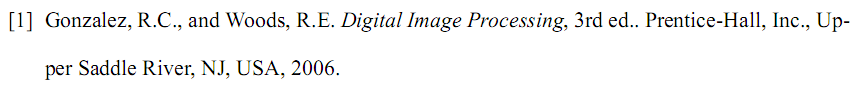
\includegraphics[width=\textwidth]{Figures/Ch2/gonzalez.png}

این شیوه برای تعداد مراجع کم بد نیست اما اگر فرمت مراجع، ترتیب یا تعداد آنها را خواسته باشید تغییر دهید، به عنوان مثال ابتدا حرف اول نام نویسنده بیاید و سپس نام خانوادگی، باید همه کارها را به صورت دستی انجام دهید.
اگر مایلید کنترل کاملی بر مراجع خود داشته باشید و به راحتی بتوانید قالب مراجع خود را عوض کنید باید از \lr{Bib\TeX} استفاده کنید که درپیوست  \ref{App:RefMan} به  آن پرداخته خواهد شد.
!
را در فایل 
\lr{IUT-Thesis.tex}،
غیرفعال%
\footnote{
	برای غیرفعال کردن یک دستور، کافی است در ابتدای آن، یک علامت
	\%
	بگذارید.
}
کنید.  در غیر این صورت، ابتدا مطالب دو فصل اول  پردازش شده و سپس مطالب فصل ۳ پردازش می‌شود و این کار باعث طولانی شدن زمان اجرا می‌شود. هر زمان که خروجی کل پروژه/پایان‌نامه/رساله خود را خواستید تمام فصلها را از حالت توضیح خارج کنید.
\subsection{مراجع}
برای وارد کردن مراجع پروژه/پایان‌نامه/رساله خود، کافی است فایل 
\lr{References.bib}
را باز کرده و مراجع خود را مانند مراجع داخل آن، وارد کنید.  سپس از \lr{bibtex} برای تولید مراجع با قالب مناسب استفاده کنید. برای توضیحات بیشتر بخش \ref{Sec:Ref} و پیوست \ref{App:RefMan} را ببینید.


%\subsection{واژه‌نامه فارسی به انگلیسی و برعکس}
%برای وارد کردن واژه‌نامه فارسی به انگلیسی و برعکس، بهتر است از بسته
%\lr{glossaries}
%استفاده کنید. راهنمای این بسته را می‌توانید به راحتی و با یک جستجوی ساده در اینترنت پیدا کنید.
%\subsection{نمایه}
%برای وارد کردن نمایه، باید از 
%\lr{xindy}
%استفاده کنید.
%زیرا 
%\lr{MakeIndex}
%با حروف «گ»، «چ»، «پ»، «ژ» و «ک» مشکل دارد و ترتیب الفبایی این حروف را رعایت نمی‌کند. همچنین، فاصله بین هر گروه از کلمات در 
%\lr{MakeIndex}،
%به درستی رعایت نمی‌شود که باعث زشت شدن حروف‌چینی این قسمت می‌شود. 
%راهنمای چگونگی کار با 
%\lr{xindy} 
%را می‌توانید در اینترنت پیدا کنید.

\section{اگر سوالی داشتم، از کی بپرسم؟}
سوالات خود در مورد نحوه استفاده از این قالب را می‌توانید از تحصیلات تکمیلی دانشکده مکانیک دانشگاه صنعتی اصفهان بپرسید. درضمن جهت ارتقا قالب حاضر و بهبود کیفیت آن، لطفا کلیه اشکالات این قالب را به تحصیلات تکمیلی دانشکده مکانیک دانشگاه صنعتی اصفهان اطلاع دهید.
همچنین برای پرسیدن سوال‌های خود موقع حروف‌چینی با زی‌پرشین،  می‌توانید به
\href{http://forum.parsilatex.com}{تالار گفتگوی پارسی‌لاتک}%
\LTRfootnote{http://forum.parsilatex.com}
مراجعه کنید. شما هم می‌توانید روزی به سوال‌های دیگران در این تالار، جواب بدهید.

\section{جمع‌بندی}
بسته‌ی زی‌پرشین و بسیاری بسته‌های مرتبط با آن مانند \lr{bidi} و \lr{Persian-bib}، مجموعه پارسی‌لاتک، مثالهای مختلف موجود در آن، استیلهای مختلف پایان‌نامه دانشگاههای مختلف، سایت پارسی‌لاتک همه به صورت داوطلبانه انجام شده‌اند. کار اصلی نوشتن و توسعه زی‌پرشین توسط آقای وفا خلیقی انجام شده است که این کار بزرگ را به انجام رساندند. همچنین متن این فصل از نوشته‌های آقای وحید امین‌طوسی در مورد نحوه نگارش پایان‌نامه اقتباس شده است.!
و
\verb!\chapter{آشنایی سریع با برخی دستورات لاتک}\label{Chap:latexIntro}
در این فصل ویژگی‌های مهم و پرکاربرد زی‌پرشین و لاتک معرفی می‌شود. برای راهنمایی بیشتر و به‌کاربردن ویژگی‌های پیشرفته‌تر به راهنمای زی‌پرشین و راهنمای لاتک مراجعه کنید. برای آگاهی از دستورات لاتک که این خروجی را تولید کرده‌اند فایل \lr{Chapter2.tex} را ملاحظه فرمایید.
\footnote{بیشتر مطالب این بخش از مثال 
	\lr{xepersian\_example.tex}
	گرفته شده‌اند که توسط دوستمان آقای امیرمسعود پورموسی آماده شده بوده است.}

\section{بندها و زیرنویس‌ها}
هر جایی از نوشته خود، اگر می‌خواهید به سر سطر بروید و یک بند تازه را آغاز کنید، باید یک خط را خالی بگذارید
\footnote{یعنی دوبار باید کلید \lr{Enter} را بزنید.}
مانند این:

حالا که یک بند تازه آغاز شده است، یک زیرنویس انگلیسی
\LTRfootnote{English Footnote!}
هم می‌نویسیم!
\section{فرمول‌های ریاضی}\label{formula}

اینجا هم یک فرمول می‌آوریم که شماره دارد:
\begin{equation}\label{eq:yek}
A=\frac{c}{d}+\frac{q^2}{\sin(\omega t)+\Omega_{12}}
\end{equation}
در لاتک می‌توان به کمک فرمان 
\lr{\textbackslash label\{\}}
به هر فرمول یک نام نسبت داد. در فرمول بالا نام \lr{eq:yek} را برایش گذاشته‌ایم (پرونده \lr{tex} همراه با این مثال را ببینید). این نام ما را قادر می‌کند که بعداً بتوانیم با فرمان
\lr{\textbackslash ref\{eq:yek\}}
به آن فرمول با شماره ارجاع دهیم. یعنی بنویسیم فرمول \ref{eq:yek}. 
لاتک خودش شماره این فرمول‌ها را مدیریت می‌کند.\footnote{یعنی اگر بعداً فرمولی قبل از این فرمول بنویسیم، خودبه‌خود شماره این فرمول و شماره ارجاع‌ها به این فرمول یکی زیاد می‌شود. دیگر نگران شماره‌گذاری فرمول‌های خود نباشید!} این هم یک فرمول که شماره ندارد:
$$A=|\vec{a}\times \vec{b}| + \sum_{n=0}^\infty C_{ij}$$

این هم عبارتی ریاضی مانند 
$\sqrt{a^2+b^2}$
که بین متن می‌آید.
\subsection{یک زیربخش}\label{zirbakhsh}

این زیربخش \ref{zirbakhsh} است؛ یعنی یک بخش درون بخش \ref{formula} است.
\subsubsection{یک زیرزیربخش}
این هم یک زیرزیربخش است. در لاتک می‌توانید بخش‌های تودرتو در نوشته‌تان تعریف کنید تا ساختار منطقی نوشته را به خوبی نشان دهید. می‌توانید به این بخش‌ها هم با شماره ارجاع دهید، مثلاً بخش فرمول‌های ریاضی شماره‌اش \ref{formula} است.
\section{نوشته‌های فارسی و انگلیسی مخلوط}
نوشتن یک کلمه انگلیسی بین متن فارسی بدیهی است، مانند 
\lr{Example}
در این جمله.
نوشتن یک عبارت چندکلمه‌ای مانند
\lr{More than one word} کمی پیچیده‌تر است.

اگر ناگهان تصمیم بگیرید که یک بند کاملاً انگلیسی را بنویسید، باید:
\begin{latin}
	This is an English paragraph from left to right. You can write as much as you want in it.
\end{latin}
\section{افزودن تصویر به نوشته}
پرونده تصویر دلخواه خود را در کنار پرونده \lr{tex} قرار دهید. سپس به روش زیر تصویر را در نوشته خود بیاورید:
\begin{latin}
	\begin{verbatim}
	\includegraphics{YourImageFileName}
	\end{verbatim}
\end{latin}
به تصویرها هم مانند فرمول‌ها و بخش‌ها می‌توان با شماره ارجاع داد. مثلاً تصویر  \ref{fig:shir} یک شیر علاقه‌مند به لاتک را در حال دویدن نشان می‌دهد. برای جزئیات بیشتر درباره روش گذاشتن تصویرها در نوشته باید راهنماهای لاتک را بخوانید.
\begin{figure}%[ht]
	\centerline{
\includegraphics[width=5cm]{Figures/Ch2/lion.jpg}}
	\caption{در این تصویر یک شیر علاقه‌مند به لاتک را در حال دویدن می‌بینید.}
	\label{fig:shir}
\end{figure}

به تصویرها هم مانند فرمول‌ها و بخش‌ها می‌توان با شماره ارجاع داد. مثلاً تصویر بالا شماره‌اش \ref{fig:shir} است. برای جزئیات بیشتر درباره روش گذاشتن تصویرها در نوشته باید راهنماهای لاتک را بخوانید.

\section{محیط‌های شمارش و نکات}
برای فهرست‌کردن چندمورد، اگر ترتیب برایمان مهم نباشد:
\begin{itemize}
	\item[-] مورد یکم
	\item[-] مورد دوم
	\item[-] مورد سوم
\end{itemize}
و اگر ترتیب برایمان مهم باشد:
\begin{enumerate}
	\item مورد یکم
	\item مورد دوم
	\item مورد سوم
\end{enumerate}
می‌توان موردهای تودرتو داشت:
\begin{enumerate}
	\item مورد ۱
	\item مورد ۲
	\begin{enumerate}
		\item مورد ۱ از ۲
		\item مورد ۲ از ۲
		\item مورد ۳ از ۲
	\end{enumerate}
	\item مورد ۳
\end{enumerate}
شماره‌گذاری این موردها را هم لاتک انجام می‌دهد.
%\section{تعریف و قضیه}
%برای ذکر تعریف، قضیه و مثال مثالهای ذیل را ببینید.
%\begin{definition}
%	مجموعه همه ارزیابی‌های  (پیوسته)  روی $(X,\tau)$، دامنه توانی احتمالی
%	\index{دامنه توانی احتمالی}
%	$ X $
%	نامیده می‌شود.
%\end{definition}
%\begin{theorem}[باناخ-آلااغلو]
%	\index{قضیه باناخ-آلااغلو}
%	اگر $ V $ یک همسایگی $ 0 $ در فضای برداری 
%	\index{فضای!برداری}
%	توپولوژیکی $ X $ باشد و 
%	\begin{equation}\label{eq1}
%	K=\left\lbrace \Lambda \in X^{*}:|\Lambda x|\leqslant 1 ; \ \forall x\in V\right\rbrace,
%	\end{equation}
%	آنگاه $ K $،  ضعیف*-فشرده است که در آن، $ X^{*} $ دوگان
%	\index{فضای!دوگان}
%	فضای برداری توپولوژیکی $ X $ است به ‌طوری که عناصر آن،  تابعی‌های 
%	خطی پیوسته
%	\index{تابعی خطی پیوسته}
%	روی $X$ هستند.
%\end{theorem}
%تساوی \eqref{eq1} یکی از مهم‌ترین تساوی‌ها در آنالیز تابعی است که در ادامه، به وفور از آن استفاده می‌شود.
%\begin{example}
%	برای هر فضای مرتب، گردایه 
%	$$U:=\left\lbrace U\in O: U=\uparrow U\right\rbrace $$
%	از مجموعه‌های بالایی باز، یک توپولوژی تعریف می‌کند که از توپولوژی اصلی، درشت‌تر  است.
%\end{example}
%حال تساوی 
%\begin{equation}\label{eq2}
%\sum_{n=1}^{+\infty} 3^{n}x+7x=\int_{1}^{n}8nx+\exp{(2nx)}
%\end{equation}
%را در نظر بگیرید. با مقایسه تساوی \eqref{eq2} با تساوی \eqref{eq1} می‌توان نتیجه گرفت که ...
%
\section{چگونگی نوشتن و ارجاع به مراجع}\label{Sec:Ref}

در لاتک به راحتی می‌توان مراجع خود را نوشت و به آنها ارجاع داد. به عنوان مثال برای معرفی کتاب گنزالس \cite{Gonzalez02book} به عنوان یک مرجع می‌توان آنرا به صورت زیر معرفی نمود:

\singlespacing
\begin{LTR}
	\begin{verbatim}
	\bibitem{Gonzalez02book}
	Gonzalez, R.C., and Woods, R.E. {\em Digital Image Processing}, 3rd ed..
	Prentice-Hall, Inc., Upper Saddle River, NJ, USA, 2006.
	\end{verbatim}
\end{LTR}
\doublespacing

در دستورات فوق \lr{Gonzalez02book}  برچسبی است که به این مرجع داده شده است و با استفاده از دستور 
\verb!\cite{Gonzalez02book}!
می‌توان به آن ارجاع داد؛ بدون این که شماره‌اش را در فهرست مراجع‌مان بدانیم.

اگر این اولین مرجع ما باشد در قسمت مراجع به صورت زیر خواهد آمد:\\
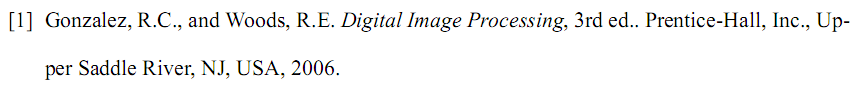
\includegraphics[width=\textwidth]{Figures/Ch2/gonzalez.png}

این شیوه برای تعداد مراجع کم بد نیست اما اگر فرمت مراجع، ترتیب یا تعداد آنها را خواسته باشید تغییر دهید، به عنوان مثال ابتدا حرف اول نام نویسنده بیاید و سپس نام خانوادگی، باید همه کارها را به صورت دستی انجام دهید.
اگر مایلید کنترل کاملی بر مراجع خود داشته باشید و به راحتی بتوانید قالب مراجع خود را عوض کنید باید از \lr{Bib\TeX} استفاده کنید که درپیوست  \ref{App:RefMan} به  آن پرداخته خواهد شد.
!
را در فایل 
\lr{IUT-Thesis.tex}،
غیرفعال%
\footnote{
	برای غیرفعال کردن یک دستور، کافی است در ابتدای آن، یک علامت
	\%
	بگذارید.
}
کنید.  در غیر این صورت، ابتدا مطالب دو فصل اول  پردازش شده و سپس مطالب فصل ۳ پردازش می‌شود و این کار باعث طولانی شدن زمان اجرا می‌شود. هر زمان که خروجی کل پروژه/پایان‌نامه/رساله خود را خواستید تمام فصلها را از حالت توضیح خارج کنید.
\subsection{مراجع}
برای وارد کردن مراجع پروژه/پایان‌نامه/رساله خود، کافی است فایل 
\lr{References.bib}
را باز کرده و مراجع خود را مانند مراجع داخل آن، وارد کنید.  سپس از \lr{bibtex} برای تولید مراجع با قالب مناسب استفاده کنید. برای توضیحات بیشتر بخش \ref{Sec:Ref} و پیوست \ref{App:RefMan} را ببینید.


%\subsection{واژه‌نامه فارسی به انگلیسی و برعکس}
%برای وارد کردن واژه‌نامه فارسی به انگلیسی و برعکس، بهتر است از بسته
%\lr{glossaries}
%استفاده کنید. راهنمای این بسته را می‌توانید به راحتی و با یک جستجوی ساده در اینترنت پیدا کنید.
%\subsection{نمایه}
%برای وارد کردن نمایه، باید از 
%\lr{xindy}
%استفاده کنید.
%زیرا 
%\lr{MakeIndex}
%با حروف «گ»، «چ»، «پ»، «ژ» و «ک» مشکل دارد و ترتیب الفبایی این حروف را رعایت نمی‌کند. همچنین، فاصله بین هر گروه از کلمات در 
%\lr{MakeIndex}،
%به درستی رعایت نمی‌شود که باعث زشت شدن حروف‌چینی این قسمت می‌شود. 
%راهنمای چگونگی کار با 
%\lr{xindy} 
%را می‌توانید در اینترنت پیدا کنید.

\section{اگر سوالی داشتم، از کی بپرسم؟}
سوالات خود در مورد نحوه استفاده از این قالب را می‌توانید از تحصیلات تکمیلی دانشکده مکانیک دانشگاه صنعتی اصفهان بپرسید. درضمن جهت ارتقا قالب حاضر و بهبود کیفیت آن، لطفا کلیه اشکالات این قالب را به تحصیلات تکمیلی دانشکده مکانیک دانشگاه صنعتی اصفهان اطلاع دهید.
همچنین برای پرسیدن سوال‌های خود موقع حروف‌چینی با زی‌پرشین،  می‌توانید به
\href{http://forum.parsilatex.com}{تالار گفتگوی پارسی‌لاتک}%
\LTRfootnote{http://forum.parsilatex.com}
مراجعه کنید. شما هم می‌توانید روزی به سوال‌های دیگران در این تالار، جواب بدهید.

\section{جمع‌بندی}
بسته‌ی زی‌پرشین و بسیاری بسته‌های مرتبط با آن مانند \lr{bidi} و \lr{Persian-bib}، مجموعه پارسی‌لاتک، مثالهای مختلف موجود در آن، استیلهای مختلف پایان‌نامه دانشگاههای مختلف، سایت پارسی‌لاتک همه به صورت داوطلبانه انجام شده‌اند. کار اصلی نوشتن و توسعه زی‌پرشین توسط آقای وفا خلیقی انجام شده است که این کار بزرگ را به انجام رساندند. همچنین متن این فصل از نوشته‌های آقای وحید امین‌طوسی در مورد نحوه نگارش پایان‌نامه اقتباس شده است.
\chapter{آشنایی سریع با برخی دستورات لاتک}\label{Chap:latexIntro}
در این فصل ویژگی‌های مهم و پرکاربرد زی‌پرشین و لاتک معرفی می‌شود. برای راهنمایی بیشتر و به‌کاربردن ویژگی‌های پیشرفته‌تر به راهنمای زی‌پرشین و راهنمای لاتک مراجعه کنید. برای آگاهی از دستورات لاتک که این خروجی را تولید کرده‌اند فایل \lr{Chapter2.tex} را ملاحظه فرمایید.
\footnote{بیشتر مطالب این بخش از مثال 
	\lr{xepersian\_example.tex}
	گرفته شده‌اند که توسط دوستمان آقای امیرمسعود پورموسی آماده شده بوده است.}

\section{بندها و زیرنویس‌ها}
هر جایی از نوشته خود، اگر می‌خواهید به سر سطر بروید و یک بند تازه را آغاز کنید، باید یک خط را خالی بگذارید
\footnote{یعنی دوبار باید کلید \lr{Enter} را بزنید.}
مانند این:

حالا که یک بند تازه آغاز شده است، یک زیرنویس انگلیسی
\LTRfootnote{English Footnote!}
هم می‌نویسیم!
\section{فرمول‌های ریاضی}\label{formula}

اینجا هم یک فرمول می‌آوریم که شماره دارد:
\begin{equation}\label{eq:yek}
A=\frac{c}{d}+\frac{q^2}{\sin(\omega t)+\Omega_{12}}
\end{equation}
در لاتک می‌توان به کمک فرمان 
\lr{\textbackslash label\{\}}
به هر فرمول یک نام نسبت داد. در فرمول بالا نام \lr{eq:yek} را برایش گذاشته‌ایم (پرونده \lr{tex} همراه با این مثال را ببینید). این نام ما را قادر می‌کند که بعداً بتوانیم با فرمان
\lr{\textbackslash ref\{eq:yek\}}
به آن فرمول با شماره ارجاع دهیم. یعنی بنویسیم فرمول \ref{eq:yek}. 
لاتک خودش شماره این فرمول‌ها را مدیریت می‌کند.\footnote{یعنی اگر بعداً فرمولی قبل از این فرمول بنویسیم، خودبه‌خود شماره این فرمول و شماره ارجاع‌ها به این فرمول یکی زیاد می‌شود. دیگر نگران شماره‌گذاری فرمول‌های خود نباشید!} این هم یک فرمول که شماره ندارد:
$$A=|\vec{a}\times \vec{b}| + \sum_{n=0}^\infty C_{ij}$$

این هم عبارتی ریاضی مانند 
$\sqrt{a^2+b^2}$
که بین متن می‌آید.
\subsection{یک زیربخش}\label{zirbakhsh}

این زیربخش \ref{zirbakhsh} است؛ یعنی یک بخش درون بخش \ref{formula} است.
\subsubsection{یک زیرزیربخش}
این هم یک زیرزیربخش است. در لاتک می‌توانید بخش‌های تودرتو در نوشته‌تان تعریف کنید تا ساختار منطقی نوشته را به خوبی نشان دهید. می‌توانید به این بخش‌ها هم با شماره ارجاع دهید، مثلاً بخش فرمول‌های ریاضی شماره‌اش \ref{formula} است.
\section{نوشته‌های فارسی و انگلیسی مخلوط}
نوشتن یک کلمه انگلیسی بین متن فارسی بدیهی است، مانند 
\lr{Example}
در این جمله.
نوشتن یک عبارت چندکلمه‌ای مانند
\lr{More than one word} کمی پیچیده‌تر است.

اگر ناگهان تصمیم بگیرید که یک بند کاملاً انگلیسی را بنویسید، باید:
\begin{latin}
	This is an English paragraph from left to right. You can write as much as you want in it.
\end{latin}
\section{افزودن تصویر به نوشته}
پرونده تصویر دلخواه خود را در کنار پرونده \lr{tex} قرار دهید. سپس به روش زیر تصویر را در نوشته خود بیاورید:
\begin{latin}
	\begin{verbatim}
	\includegraphics{YourImageFileName}
	\end{verbatim}
\end{latin}
به تصویرها هم مانند فرمول‌ها و بخش‌ها می‌توان با شماره ارجاع داد. مثلاً تصویر  \ref{fig:shir} یک شیر علاقه‌مند به لاتک را در حال دویدن نشان می‌دهد. برای جزئیات بیشتر درباره روش گذاشتن تصویرها در نوشته باید راهنماهای لاتک را بخوانید.
\begin{figure}%[ht]
	\centerline{
\includegraphics[width=5cm]{Figures/Ch2/lion.jpg}}
	\caption{در این تصویر یک شیر علاقه‌مند به لاتک را در حال دویدن می‌بینید.}
	\label{fig:shir}
\end{figure}

به تصویرها هم مانند فرمول‌ها و بخش‌ها می‌توان با شماره ارجاع داد. مثلاً تصویر بالا شماره‌اش \ref{fig:shir} است. برای جزئیات بیشتر درباره روش گذاشتن تصویرها در نوشته باید راهنماهای لاتک را بخوانید.

\section{محیط‌های شمارش و نکات}
برای فهرست‌کردن چندمورد، اگر ترتیب برایمان مهم نباشد:
\begin{itemize}
	\item[-] مورد یکم
	\item[-] مورد دوم
	\item[-] مورد سوم
\end{itemize}
و اگر ترتیب برایمان مهم باشد:
\begin{enumerate}
	\item مورد یکم
	\item مورد دوم
	\item مورد سوم
\end{enumerate}
می‌توان موردهای تودرتو داشت:
\begin{enumerate}
	\item مورد ۱
	\item مورد ۲
	\begin{enumerate}
		\item مورد ۱ از ۲
		\item مورد ۲ از ۲
		\item مورد ۳ از ۲
	\end{enumerate}
	\item مورد ۳
\end{enumerate}
شماره‌گذاری این موردها را هم لاتک انجام می‌دهد.
%\section{تعریف و قضیه}
%برای ذکر تعریف، قضیه و مثال مثالهای ذیل را ببینید.
%\begin{definition}
%	مجموعه همه ارزیابی‌های  (پیوسته)  روی $(X,\tau)$، دامنه توانی احتمالی
%	\index{دامنه توانی احتمالی}
%	$ X $
%	نامیده می‌شود.
%\end{definition}
%\begin{theorem}[باناخ-آلااغلو]
%	\index{قضیه باناخ-آلااغلو}
%	اگر $ V $ یک همسایگی $ 0 $ در فضای برداری 
%	\index{فضای!برداری}
%	توپولوژیکی $ X $ باشد و 
%	\begin{equation}\label{eq1}
%	K=\left\lbrace \Lambda \in X^{*}:|\Lambda x|\leqslant 1 ; \ \forall x\in V\right\rbrace,
%	\end{equation}
%	آنگاه $ K $،  ضعیف*-فشرده است که در آن، $ X^{*} $ دوگان
%	\index{فضای!دوگان}
%	فضای برداری توپولوژیکی $ X $ است به ‌طوری که عناصر آن،  تابعی‌های 
%	خطی پیوسته
%	\index{تابعی خطی پیوسته}
%	روی $X$ هستند.
%\end{theorem}
%تساوی \eqref{eq1} یکی از مهم‌ترین تساوی‌ها در آنالیز تابعی است که در ادامه، به وفور از آن استفاده می‌شود.
%\begin{example}
%	برای هر فضای مرتب، گردایه 
%	$$U:=\left\lbrace U\in O: U=\uparrow U\right\rbrace $$
%	از مجموعه‌های بالایی باز، یک توپولوژی تعریف می‌کند که از توپولوژی اصلی، درشت‌تر  است.
%\end{example}
%حال تساوی 
%\begin{equation}\label{eq2}
%\sum_{n=1}^{+\infty} 3^{n}x+7x=\int_{1}^{n}8nx+\exp{(2nx)}
%\end{equation}
%را در نظر بگیرید. با مقایسه تساوی \eqref{eq2} با تساوی \eqref{eq1} می‌توان نتیجه گرفت که ...
%
\section{چگونگی نوشتن و ارجاع به مراجع}\label{Sec:Ref}

در لاتک به راحتی می‌توان مراجع خود را نوشت و به آنها ارجاع داد. به عنوان مثال برای معرفی کتاب گنزالس \cite{Gonzalez02book} به عنوان یک مرجع می‌توان آنرا به صورت زیر معرفی نمود:

\singlespacing
\begin{LTR}
	\begin{verbatim}
	\bibitem{Gonzalez02book}
	Gonzalez, R.C., and Woods, R.E. {\em Digital Image Processing}, 3rd ed..
	Prentice-Hall, Inc., Upper Saddle River, NJ, USA, 2006.
	\end{verbatim}
\end{LTR}
\doublespacing

در دستورات فوق \lr{Gonzalez02book}  برچسبی است که به این مرجع داده شده است و با استفاده از دستور 
\verb!\cite{Gonzalez02book}!
می‌توان به آن ارجاع داد؛ بدون این که شماره‌اش را در فهرست مراجع‌مان بدانیم.

اگر این اولین مرجع ما باشد در قسمت مراجع به صورت زیر خواهد آمد:\\
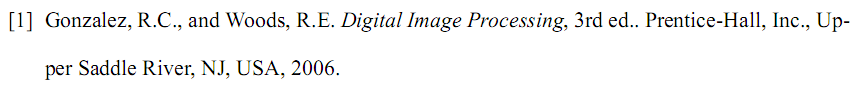
\includegraphics[width=\textwidth]{Figures/Ch2/gonzalez.png}

این شیوه برای تعداد مراجع کم بد نیست اما اگر فرمت مراجع، ترتیب یا تعداد آنها را خواسته باشید تغییر دهید، به عنوان مثال ابتدا حرف اول نام نویسنده بیاید و سپس نام خانوادگی، باید همه کارها را به صورت دستی انجام دهید.
اگر مایلید کنترل کاملی بر مراجع خود داشته باشید و به راحتی بتوانید قالب مراجع خود را عوض کنید باید از \lr{Bib\TeX} استفاده کنید که درپیوست  \ref{App:RefMan} به  آن پرداخته خواهد شد.

\chapter{امتحانی}
\section{نمرات}
سلام سلام سلام%
\LTRfootnote{hello}
\LTRfootnote{hi}
\begin{itemize}
	\item یک
	\item دو
\end{itemize}

\%13 

\begin{equation}
\frac{1}{2}
\end{equation}

$2$

مرجع های 
\cite{Amintoosi09regional,Baker02limits}

%

% ░░░░░░░▒▒▒▒▒▒▓▓▓▓ Appendices ▓▓▓▓▒▒▒▒▒▒░░░░░░░
\MakeAppendices%
\section{مدیریت مراجع در لاتک}\label{App:RefMan}
در بخش \ref{Sec:Ref} اشاره شد که با دستور 
 \lr{\textbackslash bibitem}
  می‌توان یک مرجع را تعریف نمود و با فرمان
 \lr{\textbackslash cite}
  به آن ارجاع داد. این روش برای تعداد مراجع زیاد و تغییرات آنها مناسب نیست. در ادامه به صورت مختصر توضیحی در خصوص برنامه \lr{BibTeX} که همراه با توزیع‌های معروف تِک عرضه می‌شود و نحوه استفاده از آن در زی‌پرشین خواهیم داشت.

\subsection{ مدیریت مراجع با  \texorpdfstring{\lr{Bib\TeX}}{Bib\TeX} }
یکی از روش‌های قدرتمند و انعطاف‌پذیر برای نوشتن مراجع مقالات و مدیریت مراجع در لاتک، استفاده از  \lr{BibTeX} است.
 روش کار با  \lr{BibTeX} به این صورت است که مجموعه‌ی همه‌ی مراجعی را که در پروژه/پایان‌نامه/رساله استفاده کرده یا خواهیم کرد، 
در پرونده‌ی جداگانه‌ای نوشته و به آن فایل در سند خودمان به صورت مناسب لینک می‌دهیم.
 کنفرانس‌ها یا مجله‌های گوناگون برای نوشتن مراجع، قالب‌ها یا قراردادهای متفاوتی دارند که به آنها استیلهای مراجع گفته می‌شود.
 در این حالت به کمک ‌استیل‌های \lr{BibTeX} خواهید توانست تنها با تغییر یک پارامتر در پرونده‌ی ورودی خود، مراجع را مطابق قالب موردنظر تنظیم کنید. 
 بیشتر مجلات و کنفرانس‌های معتبر یک پرونده‌ی سبک (\lr{BibTeX Style}) با پسوند \lr{bst} در وب‌گاه خود می‌گذارند که برای همین منظور طراحی شده است.

به جز نوشتن مقالات این سبک‌ها کمک بسیار خوبی برای تهیه‌ی مستندات علمی همچون پایان‌نامه‌هاست که فرد می‌تواند هر قسمت از کارش را که نوشت مراجع مربوطه را به بانک مراجع خود اضافه نماید. با داشتن چنین بانکی از مراجع، وی خواهد توانست به راحتی یک یا چند ارجاع به مراجع و یا یک یا چند بخش را حذف یا اضافه ‌نماید؛ 
مراجع به صورت خودکار مرتب شده و فقط مراجع ارجاع داده شده در قسمت کتاب‌نامه خواهندآمد. قالب مراجع به صورت یکدست مطابق سبک داده شده بوده و نیازی نیست که کاربر درگیر قالب‌دهی به مراجع باشد. 
در این جا مجموعه‌ سبک‌های بسته \lr{Persian-bib} که برای  زی‌پرشین آماده شده‌اند به صورت مختصر معرفی شده و روش کار با آن‌ها گفته می‌شود. برای اطلاع بیشتر به راهنمای بسته‌ی \lr{Persian-bib} مراجعه فرمایید.
\subsection{سبک‌های فعلی قابل استفاده در زی‌پرشین}
در حال حاضر فایلهای سبک زیر برای استفاده در زی‌پرشین آماده شده‌اند:

\singlespacing
\begin{description}
\item [\lr{unsrt-fa.bst}] این سبک متناظر با \lr{unsrt.bst} می‌باشد. مراجع به ترتیب ارجاع در متن ظاهر می‌شوند.
\item [\lr{plain-fa.bst}] این سبک متناظر با \lr{plain.bst} می‌باشد. مراجع بر اساس نام‌خانوادگی نویسندگان، به ترتیب صعودی مرتب می‌شوند.
 همچنین ابتدا مراجع فارسی و سپس مراجع انگلیسی خواهند آمد.
\item [\lr{acm-fa.bst}] این سبک متناظر با \lr{acm.bst} می‌باشد. شبیه \lr{plain-fa.bst} است.  قالب مراجع کمی متفاوت است. اسامی نویسندگان انگلیسی با حروف بزرگ انگلیسی نمایش داده می‌شوند. (مراجع مرتب می‌شوند)
\item [\lr{ieeetr-fa.bst}] این سبک متناظر با \lr{ieeetr.bst} می‌باشد. (مراجع مرتب نمی‌شوند)
\item [\lr{plainnat-fa.bst}] این سبک متناظر با \lr{plainnat.bst} می‌باشد. نیاز به بسته \lr{natbib} دارد. (مراجع مرتب می‌شوند)
\item [\lr{chicago-fa.bst}] این سبک متناظر با \lr{chicago.bst} می‌باشد. نیاز به بسته \lr{natbib} دارد. (مراجع مرتب می‌شوند)
\item [\lr{asa-fa.bst}] این سبک متناظر با \lr{asa.bst} می‌باشد. نیاز به بسته \lr{natbib} دارد. (مراجع مرتب می‌شوند)
\item[\lr{ModifiedIEEEtranFa.bst}] این سبک متناظر با نحوه ارجاع در پایان‌نامه‌های دانشگاه صنعتی اصفهان می‌باشد.
\end{description}
\doublespacing

با استفاده از استیلهای فوق می‌توانید به انواع مختلفی از مراجع فارسی و لاتین ارجاع دهید. به عنوان نمونه مرجع 
\cite{Omidali82phdThesis}
 یک نمونه پروژه دکترا (به فارسی) و مرجع 
\cite{Vahedi87} یک نمونه مقاله مجله فارسی است.
مرجع 
\cite{Amintoosi87afzayesh}  یک نمونه  مقاله کنفرانس فارسی و
مرجع 
\cite{Pedram80osool} یک نمونه کتاب فارسی با ذکر مترجمان و ویراستاران فارسی است. مرجع 
\cite{Khalighi07MscThesis} یک نمونه پروژه کارشناسی ارشد انگلیسی و
\cite{Khalighi87xepersian} هم یک نمونه متفرقه  می‌باشند.
مراجع 
\cite{Gonzalez02book,Baker02limits} 
نمونه کتاب و مقاله انگلیسی هستند.

استیل مورد استفاده در این پروژه/پایان‌نامه/رساله 
\lr{ModifiedIEEEtranFa}
است که خروجی آنرا در بخش مراجع می‌توانید مشاهده کنید.
نمونه  خروجی سبک \lr{asa-fa} در شکل \ref{fig:asafa} آمده است.

\begin{figure}[t]
\centering
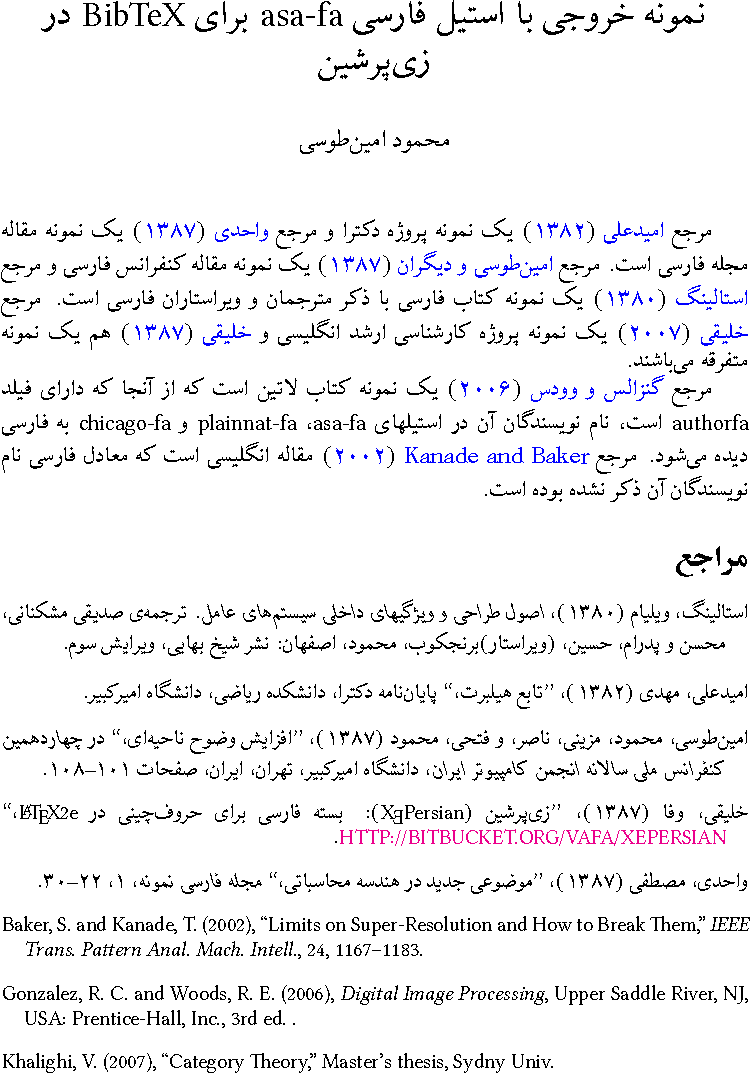
\includegraphics[width=.8\textwidth]{Figures/App1/asa-fa-crop.pdf}
\caption{نمونه خروجی با سبک \lr{asa-fa}}
\label{fig:asafa}
\end{figure} 
\subsection{ نحوه استفاده از سبک‌های فارسی}
برای استفاده از بیب‌تک باید مراجع خود را در یک فایل با پسوند \lr{bib} ذخیره نمایید. یک فایل \lr{bib} در واقع یک پایگاه داده از مراجع\LTRfootnote{Bibliography Database}  شماست که هر مرجع در آن به عنوان یک رکورد از این پایگاه داده
با قالبی خاص ذخیره می‌شود. به هر رکورد یک مدخل\LTRfootnote{Entry} گفته می‌شود. یک نمونه مدخل برای معرفی کتاب \lr{Digital Image Processing} در ادامه آمده است:

\singlespacing
\begin{LTR}
\begin{verbatim}
@BOOK{Gonzalez02image,
  AUTHOR =      {Rafael Gonzalez and Richard Woods},
  TITLE =       {Digital Image Processing},
  PUBLISHER =   {Prentice-Hall, Inc.},
  YEAR =        {2006},
  EDITION =     {3rd},
  ADDRESS =     {Upper Saddle River, NJ, USA}
}
\end{verbatim}
\end{LTR}
\doublespacing

در مثال فوق، \lr{@BOOK} مشخصه‌ی شروع یک مدخل مربوط به یک کتاب و \lr{Gonzalez02book} برچسبی است که به این مرجع منتسب شده است.
 این برچسب بایستی یکتا باشد. برای آنکه فرد به راحتی بتواند برچسب مراجع خود را به خاطر بسپارد و حتی‌الامکان برچسب‌ها متفاوت با هم باشند معمولاً از قوانین خاصی به این منظور استفاده می‌شود. یک قانون می‌تواند فامیل نویسنده‌ی اول+دورقم سال نشر+اولین کلمه‌ی عنوان اثر باشد. به \lr{AUTHOR} و $\dots$ و \lr{ADDRESS} فیلدهای این مدخل گفته می‌شود؛ که هر یک با مقادیر مربوط به مرجع مقدار گرفته‌اند. ترتیب فیلدها مهم نیست. 

انواع متنوعی از مدخل‌ها برای اقسام مختلف مراجع همچون کتاب، مقاله‌ی کنفرانس و مقاله‌ی ژورنال وجود دارد که برخی فیلدهای آنها با هم متفاوت است. 
نام فیلدها بیانگر نوع اطلاعات آن می‌باشد. مثالهای ذکر شده در فایل \lr{References.bib} کمک خوبی به شما خواهد بود. 
%این فایل یک فایل متنی بوده و با ویرایشگرهای معمول همچون \lr{Notepad++} قابل ویرایش می‌باشد. برنامه‌هایی همچون 
%\lr{TeXMaker}
% امکاناتی برای نوشتن این مدخل‌ها دارند و به صورت خودکار فیلدهای مربوطه را در فایل \lr{bib}  شما قرار می‌دهند.  
با استفاده از سبک‌های فارسی آماده شده، محتویات هر فیلد می‌تواند به فارسی نوشته شود، ترتیب مراجع و نحوه‌ی چینش فیلدهای هر مرجع را سبک مورد استفاده  مشخص خواهد کرد.

نکته: بدون اعمال تنظیمات موردنیاز \lr{Bib\TeX} در \lr{TeXWorks}، مراجع فارسی در استیل‌هایی که مراجع را به صورت مرتب شده چاپ می‌کنند، ترتیب کاملاً درستی نخواهند داشت. برای توضیحات بیشتر \cite{persianbib87userguide} را ببینید یا به سایت پارسی‌لاتک مراجعه فرمایید.

\textbf{برای درج مراجع خود لازم نیست نگران موارد فوق باشید. در فایل 
\lr{References.bib}
 که همراه با این پروژه/پایان‌نامه/رساله هست، موارد مختلفی درج شده است و کافیست مراجع خود را جایگزین موارد مندرج در آن نمایید.
}

پس از قرار دادن مراجع خود، یک بار \lr{XeLaTeX} را روی سند خود اجرا نمایید، سپس \lr{bibtex} و پس از آن دوبار \lr{XeLaTeX} را. در \lr{TeXstudio} کلید \lr{F8} و در \lr{TeXWorks} هم گزینه‌ی \lr{BibTeX} از منوی \lr{Typeset}، \lr{BibTeX} را روی سند شما اجرا می‌کنند.

برای بسیاری از مقالات لاتین حتی لازم نیست که مدخل مربوط به آنرا خودتان بنویسید. با جستجوی نام مقاله + کلمه \lr{bibtex}  در اینترنت سایتهای بسیاری همچون \lr{ACM} و \lr{ScienceDirect} را خواهید یافت که مدخل \lr{bibtex} مربوط به مقاله شما را دارند و کافیست آنرا به انتهای فایل \lr{References} اضافه کنید.

از هر یک از سبکهای \lr{Persian-bib} می‌توانید استفاده کنید، البته اگر از سه استیل آخر استفاده می‌کنید و مایلید که مراجع شما شماره بخورند باید بسته \lr{natbib} را با گزینه \lr{numbers} فراخوانی نمایید.
\newpage
\section{‌جدول، نمودار و الگوریتم در لاتک}\label{App:Latex:More}
در این بخش نمونه مثالهایی از جدول، نمودار و الگوریتم در لاتک را خواهیم دید.
\subsection{مدلهای حرکت دوبعدی}
بسیاری از اوقات حرکت بین دو تصویر از یک صحنه با یکی از مدلهای پارامتری ذکر شده در جدول \eqref{tab:MotionModels} قابل مدل نمودن می‌باشد.  
\begin{table}[ht]
	\caption{مدلهای تبدیل.}
	\label{tab:MotionModels}
	\centering
	\onehalfspacing
	\begin{tabular}{|r|c|l|r|}
		\hline نام مدل & درجه آزادی & تبدیل مختصات & توضیح \\ 
		\hline انتقالی & ۲ & $\begin{aligned} x'=x+t_x \\ y'=y+t_y \end{aligned}$  &  انتقال دوبعدی\\ 
		\hline اقلیدسی & ۳ & $\begin{aligned} x'=xcos\theta - ysin\theta+t_x \\ y'=xsin\theta+ycos\theta+t_y \end{aligned}$  &  انتقالی+دوران \\ 
		\hline مشابهت & ۴ & $\begin{aligned} x'=sxcos\theta - sysin\theta+t_x \\ y'=sxsin\theta+sycos\theta+t_y  \end{aligned}$  & اقلیدسی+تغییرمقیاس \\ 
		\hline آفین & ۶ & $\begin{aligned} x'=a_{11}x+a_{12}y+t_x \\ y'=a_{21}x+a_{22}y+t_y \end{aligned}$  & مشابهت+اریب‌شدگی \\ 
		\hline  پروجکتیو & ۸ & $\begin{aligned} x'&=(m_1x+m_2y+m_3)/D \\ y'&=(m_4x+m_5y+m_6)/D \\ D&=m_7x+m_8y+1 \end{aligned}$  & آفین+\lr{keystone+chirping} \\ 
		\hline  شارنوری & $\infty $ & $\begin{aligned} x'=x+v_x(x,y) \\ y'=y+v_y(x,y) \end{aligned}$  &  حرکت آزاد\\ 
		\hline 
	\end{tabular} 
\end{table}

\subsection{ماتریس}

شناخته‌شده‌ترین روش تخمین ماتریس هوموگرافی الگوریتم تبدیل خطی مستقیم (\lr{DLT\LTRfootnote{Direct Linear Transform}}) است.  فرض کنید چهار زوج نقطهٔ متناظر در دو تصویر در دست هستند،  $\mathbf{x}_i\leftrightarrow\mathbf{x}'_i$   و تبدیل با رابطهٔ
$\mathbf{x}'_i = H\mathbf{x}_i$
نشان داده می‌شود که در آن:
\[\mathbf{x}'_i=(x'_i,y'_i,w'_i)^\top  \]
و
\[ H=\left[
\begin{array}{ccc}
h_1 & h_2 & h_3 \\ 
h_4 & h_5 & h_6 \\ 
h_7 & h_8 & h_9
\end{array} 
\right]\]
رابطه زیر را برای الگوریتم  \eqref{alg:DLT} لازم دارم.
\begin{equation}\label{eq:DLT_Ah}
\left[
\begin{array}{ccc}
0^\top & -w'_i\mathbf{x}_i^\top & y'_i\mathbf{x}_i^\top \\ 
w'_i\mathbf{x}_i & 0^\top & -x'_i\mathbf{x}_i^\top \\ 
- y'_i\mathbf{x}_i^\top & x'_i\mathbf{x}_i^\top & 0^\top
\end{array} 
\right]
\left(
\begin{array}{c}
\mathbf{h}^1 \\ 
\mathbf{h}^2 \\ 
\mathbf{h}^3
\end{array} 
\right)=0
\end{equation}

\subsection{الگوریتم با دستورات فارسی}
با مفروضات فوق، الگوریتم \lr{DLT} به صورت نشان داده شده در الگوریتم \eqref{alg:DLT}  خواهد بود.
\begin{algorithm}[t]
	\onehalfspacing
	\caption{الگوریتم \lr{DLT} برای تخمین ماتریس هوموگرافی.} \label{alg:DLT}
	\begin{algorithmic}[1]
		\REQUIRE $n\geq4$ زوج نقطهٔ متناظر در دو تصویر 
		${\mathbf{x}_i\leftrightarrow\mathbf{x}'_i}$،\\
		\ENSURE ماتریس هوموگرافی $H$ به نحوی‌که: 
		$\mathbf{x}'_i = H \mathbf{x}_i$.
		\STATE برای هر زوج نقطهٔ متناظر
		$\mathbf{x}_i\leftrightarrow\mathbf{x}'_i$ 
		ماتریس $\mathbf{A}_i$ را با استفاده از رابطهٔ \ref{eq:DLT_Ah} محاسبه کنید.
		\STATE ماتریس‌های ۹ ستونی  $\mathbf{A}_i$ را در قالب یک ماتریس $\mathbf{A}$ ۹ ستونی ترکیب کنید. 
		\STATE تجزیهٔ مقادیر منفرد \lr{(SVD)}  ماتریس $\mathbf{A}$ را بدست آورید. بردار واحد متناظر با کمترین مقدار منفرد جواب $\mathbf{h}$ خواهد بود.
		\STATE  ماتریس هوموگرافی $H$ با تغییر شکل $\mathbf{h}$ حاصل خواهد شد.
	\end{algorithmic}
\end{algorithm}

\subsection{الگوریتم با دستورات لاتین}
الگوریتم \ref{alg:RANSAC} یک الگوریتم با دستورات لاتین است.

\begin{algorithm}[t]
	\onehalfspacing
	\caption{الگوریتم \lr{RANSAC} برای تخمین ماتریس هوموگرافی.} \label{alg:RANSAC}
	\begin{latin}
		\begin{algorithmic}[1]
			\REQUIRE $n\geq4$ putative correspondences, number of estimations, $N$, distance threshold $T_{dist}$.\\
			\ENSURE Set of inliers and Homography matrix $H$.
			\FOR{$k = 1$ to $N$}
			\STATE Randomly choose 4 correspondence,
			\STATE Check whether these points are colinear, if so, redo the above step
			\STATE Compute the homography $H_{curr}$ by DLT algorithm from the 4 points pairs,
			\STATE $\ldots$ % الگوریتم کامل نیست
			\ENDFOR
			\STATE Refinement: re-estimate H from all the inliers using the DLT algorithm.
		\end{algorithmic}
	\end{latin}
\end{algorithm}

\subsection{نمودار}
لاتک بسته‌هایی با قابلیت‌های زیاد برای رسم انواع مختلف نمودارها دارد. مانند بسته‌های \lr{Tikz} و  \lr{PSTricks}. توضیح اینها فراتر از این پیوست کوچک است. مثالهایی از رسم نمودار را در مجموعه پارسی‌لاتک خواهید یافت. توصیه می‌کنم که حتماً مثالهایی از برخی از آنها را ببینید. راهنمای همه آنها در تک‌لایو هست. نمونه مثالهایی از بسته \lr{Tikz} را می‌توانید در \url{http://www.texample.net/tikz/examples/} ببینید.

\subsection{تصویر}
نمونه تصاویری در بخش قبل دیدیم. دو تصویر شیر کنار هم را هم در شکل \ref{fig:twolion} مشاهده می‌کنید.
\begin{figure}[t]
	\centering 
	\subfloat[شیر ۱]{ \label{fig:twolion:one}
		
\includegraphics[width=.3\textwidth]{Figures/Ch2/lion.jpg}}
	%\hspace{2mm}
	\subfloat[شیر ۲]{ \label{fig:twolion:two}
		
\includegraphics[width=.3\textwidth]{Figures/Ch2/lion.jpg}}
	\caption{دو شیر}
	\label{fig:twolion} %% label for entire figure
\end{figure}%

% ░░░░░░░▒▒▒▒▒▒▓▓▓▓ References ▓▓▓▓▒▒▒▒▒▒░░░░░░░
\MakeReferences%
\bibliographystyle{Settings/ModifiedIEEEtranFa}%
\bibliography{References}%

% ░░░░░░░▒▒▒▒▒▒▓▓▓▓ Abstract - English ▓▓▓▓▒▒▒▒▒▒░░░░░░░
\DepartmentEn{Department of Mechanical Engineering}
\DegreeEn{Master of Science}%\DegreeEn{Master of Science (MSc)} % Or \DegreeEn{Doctor of Philosophy (PhD)}
\YourFullnameEn{Mohammad Jannesari}
\YourEmailAddress{m.jannesari@me.iut.ac.ir}
\DateEn{January 9, 2017}
\FirstSupervisorEn{Mahmoud Kadkhodaei, Assoc. Prof.}
\FirstSupervisorEmailAddress{kadkhodaei@cc.iut.ac.ir}
\SecondSupervisorEn{Peiman Mosaddegh, Assist. Prof.} % Optional (Remove It If You Don't Have)
\SecondSupervisorEmailAddress{mosadegh@cc.iut.ac.ir} % Optional (Remove It If You Don't Have)
\TitleEn{Finite Element Modeling of Biomechanical Behavior of \\[0.2cm] the Eye Globe Tissue by Using the Intraocular Pressure}
% اگر عنوان رساله طولانی بود، در دو خط به صورت نشان داده شده تقسیم شود.

\AbstractEn{
At this section, English abstract is written. At this section, English abstract is written. At this section, English abstract is written. At this section, English abstract is written. At this section, English abstract is written. At this section, English abstract is written. At this section, English abstract is written. At this section, English abstract is written. At this section, English abstract is written. At this section, English abstract is written. At this section, English abstract is written. At this section, English abstract is written. At this section, English abstract is written. At this section, English abstract is written. At this section, English abstract is written. At this section, English abstract is written. At this section, English abstract is written. At this section, English abstract is written. At this section, English abstract is written. At this section, English abstract is written. At this section, English abstract is written. At this section, English abstract is written. At this section, English abstract is written. At this section, English abstract is written. At this section, English abstract is written. At this section, English abstract is written. At this section, English abstract is written. At this section, English abstract is written. At this section, English abstract is written. At this section, English abstract is written. At this section, English abstract is written. At this section, English abstract is written. At this section, English abstract is written. At this section, English abstract is written. At this section, English abstract is written. At this section, English abstract is written. At this section, English abstract is written. At this section, English abstract is written. At this section, English abstract is written. At this section, English abstract is written. At this section, English abstract is written. At this section, English abstract is written. At this section, English abstract is written. At this section, English abstract is written.
}

\KeywordsEn{First Keyword, Second Keyword, Third Keyword, Fourth Keyword, Fifth Keyword}%
\MakeEnglishAbstract%

% ░░░░░░░▒▒▒▒▒▒▓▓▓▓ Signature - English ▓▓▓▓▒▒▒▒▒▒░░░░░░░
%\FirstAdvisorEn{First Advisor, Assoc. Prof.}
%\SecondAdvisorEn{Second Advisor, Assist. Prof.} % Optional (Remove It If You Don't Have)
\FirstExaminerEn{First Examiner, Assoc. Prof.} % Optional (Remove It If You Don't Have)
\SecondExaminerEn{First Examiner, Assist. Prof.} % Optional (Remove It If You Don't Have)
%\ThirdExaminerEn{Third Examiner, Prof.} % Optional (Remove It If You Don't Have)
%\FourthExaminerEn{Fourth Examiner, Prof.} % Optional (Remove It If You Don't Have)
%\FifthExaminerEn{Fifth Examiner, Prof.} % Optional (Remove It If You Don't Have)
\DeanOfDepartmentEn{Reza Tikani, Assist. Prof.}

\MakeEnglishSignaturePage%

\end{document} 

